\documentclass[11pt]{article}

\usepackage[margin=1in]{geometry}
\usepackage[T1]{fontenc}
\usepackage[utf8]{inputenc}
\usepackage{amsmath}
\usepackage{amssymb}
\usepackage{array}
\usepackage{booktabs}
\usepackage{enumitem}
\usepackage{graphicx}
\usepackage{longtable}
\usepackage[expansion=false]{microtype}
\usepackage{tikz}
\usetikzlibrary{arrows.meta,positioning}
\usepackage{hyperref}
\usepackage[numbers,sort&compress]{natbib}
\emergencystretch=2em

\newcolumntype{L}[1]{>{\raggedright\arraybackslash\sloppy}p{#1}}
\setlength{\tabcolsep}{5pt}
\renewcommand{\arraystretch}{1.12}

\hypersetup{
  colorlinks=true,
  linkcolor=blue,
  citecolor=blue,
  urlcolor=blue
}

\newcommand{\E}{\mathbb{E}}
\newcommand{\NPV}{\mathrm{NPV}}
\newcommand{\EL}{\mathrm{EL}}
\newcommand{\PPNR}{\mathrm{PPNR}}
\newcommand{\1}{\mathbf{1}}
\newcommand{\code}[1]{\nolinkurl{#1}}

\title{Credit Card Customer NPV Estimation Component:\\
A Full Evidence-Integrated Proposal for a Replacement Valuation Module}
\author{Chak Wong}
\date{July 1, 2026}

\begin{document}
\maketitle

\begin{abstract}
This report proposes a replacement net present value (NPV) estimation component
for credit-card acquisition, cross-sell, line, offer, and account-management
decisions at a large U.S. retail bank. The component is not a campaign
platform, underwriting engine, finance ledger, stress-testing system, or
reporting platform. It is the governed valuation module that those existing
systems call when they need an estimate of incremental risk-adjusted customer
value.

The proposal is intentionally full-depth. It integrates the existing literature
survey into the component design rather than replacing the survey with a short
memo. The literature body is preserved because it supplies the evidence for the
component's behavioral and financial mechanisms: household-finance and
credit-card studies show that employment, liquidity, credit limits, interest
rates, transfers, product terms, and macro shocks affect spending, borrowing,
payments, and losses; payment-choice and rewards studies show that card
adoption and card use are distinct outcomes; customer lifetime value and
duration models support lifetime activity, dormancy, and attrition modules; and
credit-risk, accounting, and supervisory sources support decomposing value into
balances, PPNR, expected loss, funding, capital, costs, and scenarios. The
proposal then translates that evidence into a practical component specification:
decision-context semantics, valuation-policy identifiers, request and response
contracts, status handling, operating modes, identification discipline,
external and internal data strategy, validation, migration, governance, and
source-support limits. Public literature supports mechanisms and model
structure; public and licensed data support scenarios, controls, benchmarks,
and priors; issuer-specific activation, cannibalization, spend response, loss
elasticity, and NPV parameters must be estimated from the bank's own data,
experiments, quasi-experiments, and reconciliations.
\end{abstract}

\section{Executive Summary and Component Charter}
\label{sec:executive-charter}

The bank's immediate task is not to build a new decisioning platform. Marketing
systems will still choose and execute campaigns; underwriting systems will
still apply credit policy; account-management systems will still execute line,
retention, conversion, and closure treatments; finance systems will still own
ledgers, planning, and official reporting; and stress-testing systems will
still own supervisory stress processes. The proposed work is narrower and more
precise: replace the current credit-card customer value component with a
governed NPV estimator that can be called by those existing systems.

The component charter is:
\begin{quote}
The NPV component owns valuation. Caller systems own action selection, policy
thresholds, campaign orchestration, underwriting rules, line-management
workflow, finance reporting, and customer execution.
\end{quote}

The component should answer three questions for every call:
\begin{enumerate}[label=\arabic*.]
  \item \textbf{What decision context is being valued?} Targeting, existing
        client cross-sell, underwriting, line assignment, offer choice, product
        conversion, retention, and portfolio analysis have different
        populations, data availability, action sets, and counterfactuals.
  \item \textbf{What valuation semantics and assumption bundle are being used?}
        A number called ``NPV'' is not useful unless horizon, discounting,
        funding, capital, tax, rewards, costs, terminal value, relationship
        value, cannibalization, macro scenario, and downstream policy
        assumptions are explicit and versioned.
  \item \textbf{What can the caller safely do with the output?} The component
        may return values, decompositions, warnings, statuses, and
        non-binding option rankings. It should not itself mail a customer,
        approve an application, choose a line, close an account, or book a
        finance result.
\end{enumerate}

The central valuation object is incremental value:
\begin{equation}
  \Delta \NPV_i(a;d,s,\pi)
  =
  \E\left[
    \NPV_i(a;d,s,\pi)-\NPV_i(a_0;d,s,\pi)
    \mid \mathcal{I}_{id}
  \right],
  \label{eq:proposal-objective}
\end{equation}
where $i$ is the customer, prospect, account, household, application, or
account-action pair being scored; $a$ is a candidate action; $a_0$ is the
decision-specific baseline; $d$ is the decision context; $s$ is the scenario
and valuation-assumption bundle; $\pi$ is the assumed downstream policy; and
$\mathcal{I}_{id}$ is the information legally and operationally available at
that decision point.

This definition prevents several common errors. A high response score is not
necessarily high value. A high first-spend account may cannibalize an old bank
card. A profitable-looking high-line decision may create exposure, capital, and
losses that offset additional interchange or finance charges. A retention or
product-conversion action may preserve value that would otherwise attrite, but
it may also give away rewards or pricing concessions to customers who would
have stayed anyway. For this reason, the component should return a tagged and
decomposed value object, not a bare scalar score.

The component must also treat card wallet as a partially observed state, not
as a directly observed label. The bank observes its own new-card transactions,
old-card transactions, deposits, debit activity, balances, payments, fees, and
losses. It usually observes competitor-card spend, competitor revolving
balances, card-on-file position, and outside payment routing only through
partial signals such as bureau attributes, balance-transfer records, payoff
records, merchant or network aggregates, account-aggregation samples, or
campaign experiments. Therefore the core modeling question is not just
``how much will the customer spend on the new card?'' It is how the action
changes the allocation of total spend, revolving balances, payment behavior,
losses, rewards cost, and relationship activity across the bank's old card, the
bank's new card, debit or deposit rails, and competitors. This distinction
separates outside wallet size, movable wallet, causal response, and NPV.

The recommended first production slice is intentionally narrow: one controlled
marketing or prescreen acquisition consumer, batch scoring, one offer family,
and one incremental pre-tax valuation semantics bundle. This permits frozen
input snapshots, campaign holdouts, shadow scoring against the current
component, portfolio-level reconciliation, and no real-time underwriting
dependency. Expansion to underwriting, line assignment, existing-account
treatments, finance planning, and account-management use cases should require
separate use-case approval.

The rest of the proposal should be read through five hard facts about card
NPV. First, NPV is latent and assumption-sensitive: it depends on long-horizon
spend, revolve, attrition, loss, funding, capital, cost, and terminal-value
assumptions that are only partially observed. Second, card value is
behaviorally heterogeneous: spend, revolve, utilization, payment behavior,
rewards response, attrition, losses, funding, and capital interact rather than
collapsing to one response or risk score. Third, the scored population changes
through the funnel from prospect to applicant to approved account to booked
and active account, so the available data and valid estimand change. Fourth,
the objective changes by decision: contact-versus-suppress,
approve-versus-decline, line-option choice, product conversion, and retention
are different counterfactuals. Fifth, decisions are sequentially
interdependent: upstream
acquisition and approval choices change downstream account populations, while
future line, pricing, retention, collections, and conversion policies change
the economics assumed upstream. These facts are the reason the component needs
decision-context declarations, valuation-semantics identifiers, decomposed
outputs, statuses, lineage, and use-case-specific validation.

\begin{figure}[t]
\centering
\resizebox{\linewidth}{!}{%
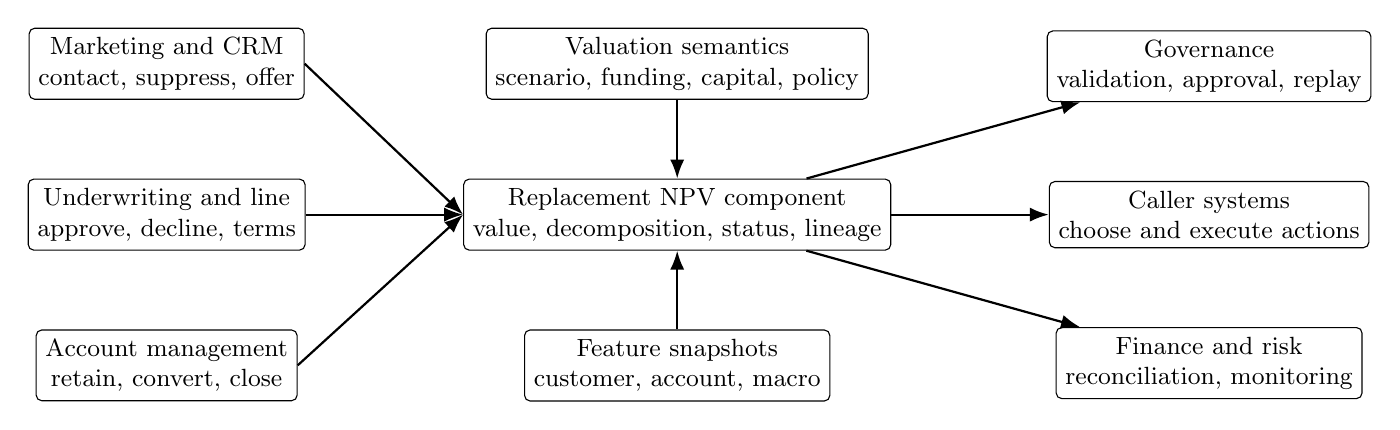
\begin{tikzpicture}[
  node distance=1.0cm and 1.2cm,
  box/.style={rectangle, draw, rounded corners=2pt, align=center,
              minimum width=3.1cm, minimum height=0.82cm, font=\small},
  wide/.style={rectangle, draw, rounded corners=2pt, align=center,
              minimum width=4.8cm, minimum height=0.9cm, font=\small},
  arr/.style={-{Latex[length=2.4mm]}, thick}
]
\node[box] (marketing) {Marketing and CRM\\contact, suppress, offer};
\node[box, below=of marketing] (uw) {Underwriting and line\\approve, decline, terms};
\node[box, below=of uw] (acct) {Account management\\retain, convert, close};

\node[wide, right=2.0cm of uw] (npv) {Replacement NPV component\\value, decomposition, status, lineage};
\node[box, above=of npv] (assump) {Valuation semantics\\scenario, funding, capital, policy};
\node[box, below=of npv] (data) {Feature snapshots\\customer, account, macro};

\node[box, right=2.0cm of npv] (owners) {Caller systems\\choose and execute actions};
\node[box, above=of owners] (gov) {Governance\\validation, approval, replay};
\node[box, below=of owners] (finance) {Finance and risk\\reconciliation, monitoring};

\draw[arr] (marketing.east) -- (npv.west);
\draw[arr] (uw.east) -- (npv.west);
\draw[arr] (acct.east) -- (npv.west);
\draw[arr] (assump) -- (npv);
\draw[arr] (data) -- (npv);
\draw[arr] (npv) -- (owners);
\draw[arr] (npv) -- (gov);
\draw[arr] (npv) -- (finance);
\end{tikzpicture}%
}
\caption{System context: the proposal replaces the valuation component, not the caller systems.}
\label{fig:system-context}
\end{figure}

\section{Replacement Boundary and How the Evidence Is Used}
\label{sec:replacement-boundary}

The current component should be inventoried before replacement. The bank should
identify all current consumers, input fields, output fields, thresholds,
fallbacks, latency classes, owners, model versions, valuation assumptions,
manual overrides, and downstream reports that depend on the current value
measure. This proposal does not assume those facts are known. It treats them as
discovery items that must be resolved before cutover.

Typical weaknesses to test in the current component are:
\begin{itemize}[leftmargin=*]
  \item response, approval, activation, or sales volume used as value proxies;
  \item unclear counterfactuals for contact, approval, line, retention, or
        product-conversion decisions;
  \item weak cannibalization treatment for existing-client new-card offers;
  \item one value definition reused across different funnel stages;
  \item missing decomposition into spend, balances, payments, PPNR, losses,
        funding, capital, rewards, fraud, servicing, and terminal value;
  \item stale discount, funding, capital, tax, cost, or reward assumptions;
  \item output fields that are difficult to reconcile to finance, risk, or
        model-risk views.
\end{itemize}

This report uses four evidence classes. First, \textbf{literature evidence}
supports mechanisms and modeling structures: income shocks affect spend,
payment instruments have adoption and use stages, rewards can change usage,
CLV models represent lifetime activity, and causal methods distinguish lift
from prediction. Second, \textbf{regulatory and supervisory sources} support a
bank-native decomposition into balances, PPNR, PD, LGD, EAD, losses, scenarios,
and controls. Third, \textbf{internal bank data} must identify proprietary
quantities that no public paper can supply: activation rates, wallet-share
capture, cannibalization, reward response, payment response, loss elasticity,
cost allocation, and terminal value. Fourth, \textbf{design conventions} make
the component auditable: valuation semantics identifiers, request lineage,
score-status handling, deterministic replay, and use-case approval.

The rest of the report is organized accordingly. Sections~\ref{sec:macro}
through~\ref{sec:validation} preserve the literature survey and modeling
framework because that evidence is the substantive basis for the component.
Sections~\ref{sec:operating-spec} through~\ref{sec:governance-migration}
translate the evidence into the actual replacement component specification.
Section~\ref{sec:audit} records source-support limits and claim use.

For readers using the document operationally, the preserved evidence body and
the new operating specification have different jobs. The evidence body explains
why the component needs state-dependent spend, separate activation and use,
cannibalization, lifetime states, PD/LGD/EAD, PPNR, and policy-dependent value.
The operating specification explains what the replacement component must expose
to other systems: decision context, valuation semantics, request and response
contracts, status handling, operating modes, migration gates, and governance
approval. The tables in the operating specification are therefore contract
summaries; the prose around them is the primary reader path.

\subsection*{Evidence-to-design spine}

To avoid a disjoint ``survey then specification'' structure, each major evidence
block should be read as answering five implementation questions. First, what
behavioral or financial mechanism does the literature support? Second, what
component requirement follows from that mechanism? Third, what internal bank
data or experiment is required before the mechanism can be parameterized for
this issuer? Fourth, which output field or decomposition item changes because
of the mechanism? Fifth, what validation or monitoring test would veto use of
that component in production? This spine is summarized as:
\[
  \text{evidence}
  \rightarrow
  \text{model requirement}
  \rightarrow
  \text{bank data}
  \rightarrow
  \text{NPV output}
  \rightarrow
  \text{validation gate}.
\]

For example, unemployment and liquidity evidence do not merely justify adding
``macro variables'' to a score. They require state-dependent purchase, payment,
balance, attrition, and loss paths, with scenario tags in the output and
macro-stress validation before use. Payment-choice evidence does not merely
say that a customer may open a card. It requires separate issuance,
activation, first-use, repeated-use, and wallet-share states, with new-card
spend kept separate from all-bank incremental spend. Credit-risk and
supervisory sources do not by themselves define campaign NPV, but they require
the valuation component to expose PD, LGD, EAD, balances, PPNR, expected loss,
funding, and capital in a form that finance, risk, and model-risk teams can
reconcile. The rest of the document follows this pattern.

\section{Introduction}

A large U.S. retail bank considering a credit card campaign faces two related
business cases. First, the bank may market a card to a prospect who is not yet a
card customer. Second, it may offer a new card to an existing client, including
an existing bank customer with deposits or loans, or an existing cardholder who
could add another card. In both cases, the operational decision is often framed
as a propensity problem: who will respond, who will be approved, who will
activate, and who will spend. That framing is useful for funnel management, but
it is incomplete for capital allocation. The economically relevant object is a
profit or value objective, not a response score alone. This is consistent with
the direct-marketing literature on optimal selection, which ranks customers by
expected net return rather than by response probability alone
\citep{bult1995directmail}, and with the customer lifetime value (CLV) and
customer-equity literatures, which define customer value as a discounted stream
of expected future contribution \citep{berger1998clv,rust2004return,venkatesan2004clv}.
The credit-card setting adds bank-specific components---losses, capital,
funding, fraud, rewards, and cannibalization---to this familiar marketing
objective.

Let $i$ index customers, $t$ monthly time, and $a \in \mathcal{A}$ a marketing
or product action, such as a direct-mail offer, digital preapproval, branch
offer, balance-transfer campaign, rewards bonus, or product upgrade. In the
direct-mail formulation, the bank would mail customer $i$ when expected margin
times response probability exceeds contact cost:
\begin{equation}
  d_i^*
  =
  \1\{p_i m_i - c_i > 0\},
  \label{eq:direct-mail-profit}
\end{equation}
where $p_i$ is response probability, $m_i$ is conditional gross margin, and
$c_i$ is contact cost. In a CLV formulation, customer value is instead a
discounted contribution stream:
\begin{equation}
  \mathrm{CLV}_i
  =
  \E\left[
    \sum_{t=0}^{T} \delta_t \{R_{it}-C_{it}\}
    \,\middle|\, \mathcal{I}_{i0}
  \right].
  \label{eq:generic-clv}
\end{equation}
The card-acquisition problem combines these ideas with treatment effects:
\begin{align}
  \Delta CF_{i,t+h}(a,\pi;s)
  &=
  \Delta PPNR_{i,t+h}(a,\pi;s)
  - \Delta EL_{i,t+h}(a,\pi;s)
  - \Delta Kchg_{i,t+h}(a,\pi;s)
  \nonumber\\
  &\quad
  - \Delta Tax_{i,t+h}(a,\pi;s)
  + \Delta RelValue_{i,t+h}(a,\pi;s),
  \label{eq:incremental-cash-flow}\\
  \Delta \NPV_i(a;d,s,\pi)
  &=
  - C_i^{\mathrm{acq}}(a)
  +
  \E\left[
    \sum_{h=0}^{H}
      \delta_h\,\Delta CF_{i,t+h}(a,\pi;s)
    + \delta_H\Delta TV_{i,t+H}(a,\pi;s)
    \,\middle|\, \mathcal{I}_{id}
  \right].
  \label{eq:incremental-npv}
\end{align}
Here $\Delta CF$ is the one-period incremental cash-flow primitive,
$\Delta PPNR$ is pre-provision net revenue, $\Delta EL$ is expected credit loss
net of recovery, $\Delta Kchg$ is a priced capital or balance-sheet charge,
$\Delta Tax$ is the tax effect under the declared valuation convention,
$\Delta RelValue$ is approved relationship-value spillover, $C_i^{\mathrm{acq}}$
is one-time acquisition or setup cost, and $\Delta TV$ is terminal value. The
increments are measured against the decision-specific baseline action $a_0$,
under scenario and valuation bundle $s$, downstream policy $\pi$, and the
information set $\mathcal{I}_{id}$ available at decision context $d$.

Thus, Equation~\eqref{eq:incremental-npv} is not claimed to be a single
canonical equation from one credit-card paper. It is the synthesis needed for a
bank: Equation~\eqref{eq:direct-mail-profit} contributes the expected-profit
targeting logic, Equation~\eqref{eq:generic-clv} contributes the discounted
lifetime stream, and causal/uplift methods contribute the requirement that all
terms be incremental to the no-offer counterfactual.

\subsection*{Four Layers of the Valuation Problem}

The proposal uses four distinct layers. The \emph{identity layer} defines
cash-flow and stock-flow accounting objects such as
Equation~\eqref{eq:incremental-cash-flow}; it must reconcile to finance and
risk definitions. The \emph{causal layer} estimates the effect of actions on
observable short- and medium-horizon outcomes, such as response, activation,
spend source, balance build, payment behavior, attrition, and loss. The
\emph{forecast layer} projects state transitions and cash-flow drivers under a
declared scenario and current state. The \emph{policy-value layer} evaluates
the discounted path under downstream account-management policy $\pi$, including
future line, repricing, retention, collections, closure, hardship, and
conversion rules. A module may be predictive without being causal, or causal
over a short horizon without by itself identifying long-horizon policy value;
the component contract should say which layer each output supports.

This counterfactual is crucial. For an existing client, observed post-campaign
spend on a new card can be high even when incremental NPV is low: the card may
shift spend from the bank's old card, pull forward spend through a costly
promotion, or create balances whose losses exceed finance charges. Conversely, a
moderate activation probability can be valuable if it creates durable
incremental purchase volume, profitable revolving balances, and low servicing
and loss costs. The bank's literature problem is therefore not a search for a
single ``credit-card NPV paper.'' It is a synthesis problem across household
finance, payment choice, credit-card economics, causal marketing, and customer
lifetime value.

This paper is organized around three questions. Section~\ref{sec:macro}
reviews evidence on how market conditions, employment, income, and liquidity
alter spending and card economics. Section~\ref{sec:usage} reviews adoption,
activation, rewards, and use of new payment instruments. Section~\ref{sec:ltv}
reviews customer lifetime value and duration models for lifetime expenditure.
Section~\ref{sec:architecture} proposes a practical model architecture for a
bank. Section~\ref{sec:component-decomposition} develops a component
decomposition into losses, balances, PPNR, and portfolio-management overlays.
Section~\ref{sec:decision-pitfalls} addresses measurement and decision
pitfalls that arise when NPV is used across the card funnel.
Section~\ref{sec:validation} discusses empirical design and validation.
Section~\ref{sec:identification-data} develops the endogeneity, selection, and
data strategy required to make the component defensible.
Section~\ref{sec:audit} records the source-support limits of this first-pass
survey.

\section{Integrated Design of the Replacement NPV Component}
\label{sec:integrated-design}

This section states the proposal in build terms before the detailed evidence
sections. The replacement is a valuation component that converts a declared
decision context, a candidate action, a customer state, product terms,
scenario assumptions, and downstream policy assumptions into a decomposed
incremental NPV object. The component must be modular because card value is
not generated by one behavior. It is generated by a linked path of adoption,
spend, payments, balances, losses, rewards, funding, capital, servicing,
attrition, and relationship effects.

For every module, the design rule is the same. The public literature or
supervisory source identifies a mechanism and a modeling slot. The bank's
internal data or experiment estimates the issuer-specific parameter. The
component exposes the resulting path or cash-flow driver in the NPV response.
Validation determines whether that module may be used for a given decision
context. This is the practical meaning of evidence integration in this
proposal.

\subsection{Module 1: spend, macro, and employment state}
\label{subsec:module-spend-macro}

The spend module forecasts purchase volume, transaction count, ticket size,
and merchant-category mix under the declared action and macro scenario. The
literature on unemployment, income shocks, liquidity, and macro disruptions
supports the mechanism that spending is state dependent. The component
therefore should not use a static average spend curve for all campaign
conditions. It should condition on customer liquidity, payroll or deposit
signals where permitted, utilization, local labor-market variables, rates,
inflation, and scenario tags.

The bank must estimate how those variables map into its own card spend,
payment rate, balance build, and attrition. Public papers can justify including
unemployment or liquidity states; they cannot identify this bank's category
spend elasticity or routing share to the new card. The output implication is
that NPV responses should expose spend and interchange by category and horizon,
plus scenario sensitivity. The validation implication is that macro backtests,
time-based holdouts, and segment calibration can veto the spend module even if
average first-spend prediction is strong.

\subsection{Module 2: new-card adoption, activation, use, and cannibalization}
\label{subsec:module-adoption-use}

The adoption and usage module separates offer response, application or
acceptance, approval where relevant, booking, activation, first use, repeated
use, wallet-share capture, dormancy, attrition, and charge-off. Payment-choice
and rewards evidence supports the distinction between having a payment
instrument and using it. It also supports modeling rewards and promotions as
treatments that can change activation, spend, debt, and reactivation.

For existing clients, the core output is not raw new-card spend. The component
must distinguish new-card spend, all-bank incremental card spend, debit or
deposit substitution where observed, old-bank-card cannibalization, and
uncertain outside-card or new-consumption components. The bank must estimate
these quantities using randomized holdouts, campaign experiments, or credible
quasi-experimental designs. The response object should label activation,
first-use probability, repeated-use probability, new-card spend lift,
all-bank-spend lift, reward cost, balance lift, loss lift, and
cannibalization. A model that predicts new-card spend but cannot identify
incremental all-bank value should remain diagnostic for cross-sell decisions.

For prospect acquisition and existing-client cross-sell, the module should also
estimate an outside-wallet state and an offer-specific movable-wallet state.
Outside wallet is the customer's spend or revolving balance not currently on
the bank's card products. Movable wallet is the fraction of that outside wallet
that the specific offer can plausibly move to the bank over the declared
horizon. It should depend on product terms, rewards, promotional duration,
channel, card-on-file friction, relationship depth, segment, macro state, and
time since offer. The component should expose whether outside-wallet and
movable-wallet quantities are directly observed, internally anchored,
externally benchmarked, experimentally identified, quasi-experimental,
model-imputed, or scenario-only.

\subsection{Module 3: lifetime state, attrition, dormancy, and terminal value}
\label{subsec:module-lifetime}

The lifetime module turns early behavior into a state path. A card customer
can be a transactor, revolver, promotional borrower, cash-advance user,
dormant account, retained account, converted account, delinquent account, or
charged-off account. CLV, customer-base, and duration models support the use
of transaction frequency, recency, monetary value, active-state inference, and
relationship duration, but card NPV must extend those models to balances,
losses, rewards, funding, and servicing.

The component should estimate transition probabilities among these states and
carry state-specific terminal-value assumptions. Terminal value should not be
one hidden scalar multiple; it should depend on state, vintage, months on book,
product, relationship depth, risk, macro state, and downstream policy. The
bank must validate lifetime state forecasts with vintage holdouts, dormancy
calibration, attrition calibration, and terminal-value sensitivity. If terminal
value dominates rankings, the response should expose that fact as a sensitivity
or warning.

\subsection{Module 4: balances, payments, lines, promotions, and cash advances}
\label{subsec:module-balances}

The balance module enforces stock-flow consistency. Purchases, cash advances,
balance transfers, fees, interest, payments, credits, charge-offs, and
adjustments should reconcile to statement and principal balances. Credit line,
APR, promo duration, balance-transfer terms, rewards, and disclosures are
candidate action terms, not passive descriptors. They can change both revenue
and risk through utilization, revolve behavior, payment rates, and EAD.

The bank must estimate line and term response from its own account history,
experiments, policy changes, and approved quasi-experimental variation. The
component output should report line, utilization, purchase balances,
cash-advance balances, balance-transfer balances, promotional balances,
payments, finance charges, fees, funding cost, and balance-linked EAD. A
balance forecast that violates stock-flow accounting or mixes principal and
non-principal balances should fail component validation.

\subsection{Module 5: losses, PD, LGD, EAD, vintage, and balance subledgers}
\label{subsec:module-losses}

The loss module uses the bank-standard PD/LGD/EAD vocabulary, but it must be
connected to the card lifecycle. PD should be a transition or hazard over
delinquency and charge-off states. LGD should reflect recovery, collections,
bankruptcy, hardship programs, and macro state. EAD should be linked to
balances, line, utilization, cash advances, balance transfers, accrued fees,
interest, and undrawn draw behavior.

The component should expose expected loss and its drivers by horizon and
option. It should also preserve vintage, months-on-book, and
principal/non-principal balance dimensions, because newly booked accounts
season differently and promotions can shift both timing and composition of
loss. Public credit-risk literature supports the structure, but the bank must
validate calibration and treatment response using internal vintages, booked
account outcomes, line-policy tests, and stress periods. A line or promo
option should not be ranked on revenue unless the linked EAD, PD, LGD, capital,
and downside risk paths are also valid.

\subsection{Module 6: PPNR, rewards, funding, capital, tax, cost, and relationship value}
\label{subsec:module-ppnr}

The finance module converts behavior into cash flows. It should decompose
incremental value into net interest income, non-interest income, non-interest
expense, expected loss, capital cost, tax treatment, acquisition cost, terminal
value, and approved relationship value. PPNR and stress-testing sources
support separating balances, revenue, expense, and losses under scenarios; CLV
literature supports discounting future contribution; bank governance requires
the decomposition to reconcile to finance and risk definitions.

Rewards, signup bonuses, servicing, fraud, disputes, collections, charge-off
sale economics, funding, liquidity, capital, and tax must not be afterthoughts.
They are often what turns high spend into low or negative value. Deposit or
other-product value should be included only when the card action is credibly
causal for relationship change; otherwise it should be excluded or reported
separately. The component should expose both the decomposed contribution path
and the valuation-semantics identifier that defines discounting, funding,
capital, tax, cost allocation, terminal value, and relationship-value rules.

\subsection{Module 7: sequential policy dependence}
\label{subsec:module-policy}

The component must tag the downstream policy assumed when valuing an action.
Acquisition value depends on future approval, line, repricing, retention,
collections, closure, and conversion policies. Underwriting and line choices
change the population and state distribution that account-management systems
later see. Account-management changes can invalidate upstream acquisition NPV
if the old model assumed different future treatment rules.

The practical requirement is a downstream-policy assumption bundle. Each NPV
response should state which policy bundle was used, and each production use
case should be approved for that bundle. If the bank changes line-management,
collections, retention, closure, or conversion policy, upstream NPV should be
revalidated. This keeps the component from optimizing a future operating world
the bank no longer runs.

\subsection{How the modules connect to caller systems}
\label{subsec:modules-to-callers}

Caller systems do not need to know every internal model detail, but they must
receive a value object whose meaning is safe for their decision. A marketing
caller needs contact-versus-suppress value, campaign cost, response and
activation lift, cannibalization, expected loss, and portfolio constraints. An
underwriting caller needs approve-versus-decline or approve-with-terms value
under credit policy, with loss, capital, compliance, and adverse-action
boundaries handled by the caller. A line-assignment caller needs option-level
value, usage, utilization, EAD, loss, capital, and status for each feasible
line. An existing-account treatment caller needs forward value under retention,
conversion, promo, closure, or no-treatment alternatives. Finance and risk
consumers need decompositions for reconciliation, not authority to treat the
component as the official ledger, CECL, or stress platform.

This is why the operating contracts later in the document exist. They are not
the product. They are the guardrails that keep a sophisticated but fragile NPV
estimate from becoming a misleading universal score.

\section{Market Conditions, Employment, and Propensity to Spend}
\label{sec:macro}

\subsection{Income, unemployment, and liquidity}

The first component of credit-card NPV is the customer's capacity and propensity
to spend. The relevant empirical papers do not estimate the bank's
Equation~\eqref{eq:incremental-npv} directly. They estimate causal or
quasi-causal effects of income, employment, and liquidity variables on spending
or debt. Their contribution to our model is a set of state variables and
elasticities for the spend, balance, and risk modules.

\citet{ganong2019unemployment} use de-identified bank account data to study
spending around unemployment and the predictable income drop at unemployment
insurance exhaustion. A stylized event-study version of the object is
\begin{equation}
  y_{i\tau}
  =
  \alpha_i + \lambda_\tau
  + \sum_{k \neq -1} \beta_k \1\{\tau_i = k\}
  + \varepsilon_{i\tau},
  \label{eq:unemployment-event-study}
\end{equation}
where $y_{i\tau}$ is spending for household $i$ at event time $\tau$ relative to
an unemployment or benefit-exhaustion event, $\alpha_i$ absorbs household fixed
effects, and the $\beta_k$ trace the spending path around the event. The
important modeling implication is not merely ``unemployment matters.'' It is
that the card spend forecast should include event-time variables such as job
loss, payroll interruption, benefit receipt, and benefit exhaustion, because
spend can move non-smoothly around predictable income events.

\citet{johnson2004rebates} study the 2001 tax rebates using variation in rebate
timing. A stylized specification is
\begin{equation}
  \Delta c_{it}
  =
  \alpha_i + \lambda_t
  + \gamma\,\mathrm{Rebate}_{it}
  + \eta' H_i\,\mathrm{Rebate}_{it}
  + u_{it},
  \label{eq:rebate-mpc}
\end{equation}
where $\gamma$ is a marginal propensity to consume out of the transfer and
$H_i$ contains heterogeneity variables such as income or liquid-wealth status.
For a credit-card model, this says that transfers, payroll changes, and liquid
wealth proxies should enter monthly purchase-volume and payment-rate equations,
with heterogeneous effects. It does not identify the share of extra consumption
that will route through our card.

\citet{gross2001liquidity} provide the closest direct credit-card evidence.
They study account-level card and bureau data and estimate how debt responds to
credit limits and interest rates. A stylized account-level equation is
\begin{equation}
  \Delta B_{it}
  =
  \alpha_i + \lambda_t
  + \theta\,\Delta \mathrm{Limit}_{it}
  + \rho\,\Delta \mathrm{APR}_{it}
  + \psi' X_{it}
  + e_{it},
  \label{eq:limit-apr-response}
\end{equation}
with stronger responses among initially high-utilization or liquidity-constrained
borrowers. This should enter our future model through the balance and payment
modules: line assignment and APR are not passive controls; they are treatment
components that affect revolving balances, utilization, finance charges, and
expected loss.

\subsection{Rates, regulation, and product terms}

Credit-card NPV is also shaped by prices, fees, disclosures, repayment rules,
and regulatory constraints. \citet{agarwal2013cardact} study the Credit Card
Accountability Responsibility and Disclosure Act using a large account-level
card panel. The paper is not a spend-propensity model, and this survey should
not use it as if it supplied a universal activation or balance elasticity. Its
modeling value is different: it shows that product terms are governed economic
objects. Fees, disclosures, and repayment nudges can change both issuer revenue
components and consumer repayment behavior, so the NPV model cannot treat APRs,
fees, and promotional terms as free scalar revenue add-ons.

Formally, the campaign action should be represented as a vector of product
terms, not as a binary contact flag:
\begin{equation}
  a_{it}
  =
  \left(
    \ell_{it}, r^{\mathrm{purchase}}_{it},
    r^{\mathrm{cash}}_{it}, r^{\mathrm{BT}}_{it},
    r^{\mathrm{promo}}_{it}, T^{\mathrm{promo}}_{it},
    f_{it}, q_{it}, b_{it}, d_{it}
  \right)
  \in \mathcal{A}_{it}(X_{it},M_{gt},G_t).
  \label{eq:offer-vector}
\end{equation}
Here $\ell$ is the credit line; the $r$ terms are purchase, cash-advance,
balance-transfer, and promotional APRs; $T^{\mathrm{promo}}$ is promotional
duration; $f$ is the vector of annual, late, balance-transfer, cash-advance,
foreign-transaction, and waiver terms; $q$ is the reward earn or redemption
schedule; $b$ is a signup or statement-credit bonus; and $d$ is the disclosure,
minimum-payment, autopay, and digital-wallet provisioning design. The feasible
set $\mathcal{A}_{it}$ is indexed by customer state, macro state, and governance
state $G_t$ because underwriting policy, compliance rules, disclosure
requirements, risk appetite, pricing floors, and operational constraints limit
which offers can be made.

This notation connects the CARD Act evidence to the later NPV architecture in
two ways. First, regulation changes the feasible set and sometimes the cash-flow
mapping:
\begin{align}
  a_{it} &\in \mathcal{A}_{it}(G_t), \label{eq:regulated-action-set}\\
  CF_{i,t+1} &= c(Z_{it},X_{it},M_{gt},a_{it};G_t).
       \label{eq:regulated-cashflow-map}
\end{align}
A rule change, fee cap, disclosure change, or repayment-allocation rule is
therefore not merely an external dummy variable. It changes either the offers
available to the bank or the function that maps behavior into interest, fees,
payments, and balances. Second, product terms are treatments that enter the
behavioral transition system. A reduced-form version is
\begin{align}
  \Pr(Z_{i,t+1}=z'\mid Z_{it},X_{it},M_{gt},a_{it},G_t),
       \label{eq:terms-transition}\\
  \E[Y_{i,t+1}\mid Z_{i,t+1},X_{it},M_{gt},a_{it},G_t],
       \qquad
  Y\in\{S,B,Pay,D,Q\}.
       \label{eq:terms-outcomes}
\end{align}
Thus APR, line, fees, rewards, and disclosures can affect activation, purchase
volume, revolving balances, payments, delinquency, rewards liability, servicing
cost, and attrition. They should not be appended only after a response model has
already selected customers.

The mathematical bridge to \citet{gross2001liquidity} is direct. Equation
\eqref{eq:limit-apr-response} says that limit and APR changes can move card
debt, especially for liquidity-constrained accounts. In the NPV engine, the
same terms must feed both revenue and risk:
\begin{align}
  B_{i,t+1}
    &=
      g_B(B_{it},Pay_{it},S_{it},\ell_{it},r_{it},f_{it},
          X_{it},M_{gt}) + \varepsilon^B_{i,t+1},
      \label{eq:terms-balance}\\
  Int_{i,t+1}
    &=
      r^{\mathrm{revolve}}_{it}\,
      B^{\mathrm{revolve}}_{i,t+1}
      + r^{\mathrm{cash}}_{it}\,
      B^{\mathrm{cash}}_{i,t+1}
      + r^{\mathrm{BT}}_{it}\,
      B^{\mathrm{BT}}_{i,t+1},
      \label{eq:terms-interest}\\
  EL_{i,t+1}
    &=
      PD_{i,t+1}(Z_{it},\mathrm{Util}_{it},X_{it},M_{gt},a_{it})\,
      LGD_{i,t+1}\,
      EAD_{i,t+1}(B_{i,t+1},\ell_{it},a_{it}).
      \label{eq:terms-loss}
\end{align}
Raising APR can mechanically increase the rate applied to revolving balances,
but it can also change borrowing, payment, attrition, and default behavior.
Increasing the line can raise usage and finance revenue, but it can also raise
utilization dynamics, exposure at default, capital, and downside risk. The
correct object for decisioning is therefore a total derivative of value with
respect to the governed offer vector, not a partial revenue calculation holding
behavior fixed. Let
$\mu_Y(a)=\E[Y_i(a)\mid\mathcal{I}_{it}]$ for
$Y\in\{Z,S,B,Pay,D,Q\}$. For any feasible local perturbation $v$ of the offer
vector,
\begin{align}
  D_v\E[\Delta \NPV_i(a)]
  &=
  \left.
  \nabla_a \E[\Delta \NPV_i(a,\mu)]^\top v
  \right|_{\mu=\mu(a)}
  \nonumber\\
  &\quad
  +
  \sum_{Y\in\{Z,S,B,Pay,D,Q\}}
  \left.
  \frac{\partial \E[\Delta \NPV_i(a,\mu)]}{\partial \mu_Y}
  \right|_{\mu=\mu(a)}
  D_v\mu_Y(a).
  \label{eq:terms-total-derivative}
\end{align}
The first term is the mechanical cash-flow effect of the term sheet; the second
term is the behavioral response channel. The second term is precisely why the
rates and regulation literature belongs before the usage, CLV, loss, balance,
and PPNR sections.

This also clarifies how product terms should be validated. The promotion
criterion is not whether a high-APR or high-fee offer raises modeled revenue
conditional on the same balance path. It is whether the feasible offer
$a\in\mathcal{A}_{it}(G_t)$ increases counterfactual value after behavioral
response, regulation, cannibalization, expected loss, capital, funding, rewards,
and servicing:
\begin{align}
  \Delta \NPV_i(a;G_t)
  &=
  -\Delta C_i^{\mathrm{acq}}(a)
  +
  \sum_{h=0}^{H}\delta_h\,
  \E\!\left[
    \Delta CF^{\mathrm{terms}}_{i,t+h}(a;G_t)
    \mid \mathcal{I}_{it}
  \right],
  \label{eq:terms-to-npv}\\
  \Delta CF^{\mathrm{terms}}_{i,t+h}(a;G_t)
  &=
  \Delta PPNR_{i,t+h}(a;G_t)
  - \Delta EL_{i,t+h}(a;G_t)
  - \Delta K_{i,t+h}(a;G_t)
  + \Delta RelValue_{i,t+h}(a).
\end{align}
Equation~\eqref{eq:terms-to-npv} is the handoff to the component decomposition
in Section~\ref{sec:component-decomposition}: promotional APRs and
balance-transfer terms become promo states and balance subledgers; fees and
waivers become non-interest income; rewards become expense and liability;
APR/line choices affect balances, EAD, and capital; disclosure and repayment
design enter payment and attrition transitions; and all terms remain subject to
the feasible governed action set.

\subsection{Macro shocks and category substitution}

Market shocks can change not only the level of spending but also the composition
of card spending. \citet{baker2020epidemic} use transaction-level household
financial data to study consumption during the COVID-19 shock. Their evidence
documents large changes in spending levels and categories during the epidemic.
For card NPV, category shifts matter because merchant-category mix affects
interchange, rewards expense, fraud risk, dispute rates, and charge-off
correlation. A recession, health shock, inflation shock, or local labor-market
shock can lower discretionary purchase volume while increasing borrowing demand
and credit risk.

The practical lesson is that spend models should be time varying and
category-aware. A customer with high pre-campaign grocery and travel spend is
not equally valuable in every macro state. A useful reduced-form component is
\begin{equation}
  \log(1+S_{ij,t+1})
  =
  \mu_i + \lambda_t + \kappa_j
  + \beta_j' M_{gt}
  + \chi_j' X_{it}
  + \omega_j' (M_{gt}\times X_{it})
  + \epsilon_{ij,t+1},
  \label{eq:category-spend}
\end{equation}
where $S_{ij,t+1}$ is spend in merchant category $j$, $M_{gt}$ is a local or
national macro vector for geography $g$, and $X_{it}$ includes customer
liquidity, payroll, utilization, and relationship variables. Equation
\eqref{eq:category-spend} is not lifted from one paper; it is the model slot
suggested by the income, liquidity, and macro-shock evidence.

\begin{table}[t]
\centering
\caption{How Section~\ref{sec:macro} evidence should enter a bank model.}
\label{tab:macro-to-model}
\begin{tabular}{p{0.22\linewidth}p{0.31\linewidth}p{0.37\linewidth}}
\toprule
Literature & Mathematical object & Model use \\
\midrule
\citet{ganong2019unemployment}
  & Event-time spending path around unemployment and benefit exhaustion.
  & Add job-loss, payroll interruption, benefit receipt, and exhaustion
    indicators to spend, payment, attrition, and loss modules. \\
\citet{johnson2004rebates}
  & Marginal propensity to consume out of transfer timing, with heterogeneity.
  & Add income/transfer shocks and liquidity interactions to spend and payment
    equations; do not assume routing to our card. \\
\citet{gross2001liquidity}
  & Account-level response of card debt to credit limits and APR.
  & Treat line and APR as treatment components affecting balances, finance
    revenue, utilization, and loss. \\
\citet{agarwal2013cardact}
  & Regulation-induced changes in fees, disclosures, repayment behavior, and
    issuer revenue components.
  & Treat APRs, fees, rewards, disclosures, and repayment rules as governed
    terms $a_{it}\in\mathcal{A}_{it}(G_t)$ that feed transition, balance, loss,
    PPNR, and promo-state equations rather than unconstrained revenue levers. \\
\citet{baker2020epidemic}
  & Transaction-level response of spending levels and categories to a macro
    shock.
  & Forecast category-level spend and interchange/rewards/fraud mix under
    macro scenarios. \\
\bottomrule
\end{tabular}
\end{table}

\subsection{Implication for the NPV component}
\label{subsec:macro-component-implication}

The macro and employment evidence should be incorporated as a dynamic state
requirement, not as a cosmetic scenario overlay. The replacement component
should carry macro, local labor-market, rate, inflation, payroll, benefit, and
liquidity variables into the spend, payment, balance, attrition, and loss
modules. It should also return the scenario identifier and sensitivity of
major NPV components to macro assumptions. For marketing and cross-sell, this
means the model must distinguish customers whose expected value comes from
durable purchase volume from customers whose value depends on fragile revolve
or liquidity stress. For line and offer decisions, it means the line, APR, and
promo terms must be modeled as actions that can change both revenue and EAD,
not as exogenous descriptors.

The public literature does not supply this bank's elasticity of card spend,
payment rate, or default to unemployment and liquidity shocks. Those
parameters require issuer transaction data, bureau refreshes, payroll or
deposit signals where permitted, campaign holdouts, and vintage backtests. The
output implication is concrete: the response object should expose category
spend, balances, payments, utilization, PD, LGD, EAD, expected loss, and PPNR
by scenario and horizon. The validation implication is equally concrete:
macro-stress backtests, local labor-market drift monitoring, and segment-level
calibration can veto use of a model even when average response or spend
prediction is strong.

\section{Will the Newly Issued Card Be Used?}
\label{sec:usage}

\subsection{Adoption is not usage}

The second requested problem is the probability that a customer who receives a
new card will use that card. The payment-choice literature warns against
collapsing this into a single response probability. \citet{koulayev2012payment}
estimate a structural model of adoption and use of payment instruments by U.S.
consumers. Their central relevance here is that possession of a payment
instrument and use of that instrument are distinct choices. A customer may open
a card, activate it, and still use another issuer's card, debit card, cash, ACH,
or a digital wallet at the point of sale.

Mathematically, the useful structure is a two-stage adoption/use problem. A
stylized version is:
\begin{align}
  A_{im}^*
    &= Z_i'\alpha_m + \nu_{im}, \qquad
       A_{im} = \1\{A_{im}^*>0\}, \label{eq:adoption-latent}\\
  U_{ijm}
    &= X_{ijm}'\beta_m + \phi_m A_{im} + \varepsilon_{ijm},
       \qquad
       m^*_{ij}=\arg\max_{m \in \mathcal{M}_i} U_{ijm}.
       \label{eq:use-utility}
\end{align}
Here $A_{im}$ denotes whether consumer $i$ has adopted payment instrument $m$,
$U_{ijm}$ is the utility of using instrument $m$ for transaction context $j$,
and $\mathcal{M}_i$ is the set of adopted instruments available to consumer
$i$. The exact specification in \citet{koulayev2012payment} is richer, but
Equations~\eqref{eq:adoption-latent}--\eqref{eq:use-utility} capture the
modeling lesson for us: ``has the card'' gates the choice set, while ``uses the
card'' is a conditional payment-choice decision. Our card model should therefore
estimate activation and usage conditional on the customer's competing payment
portfolio rather than treating issuance as usage.

For a credit-card campaign, the operational funnel should therefore separate:
\begin{enumerate}[label=\arabic*.]
  \item offer exposure and response;
  \item application and approval;
  \item card opening and physical or digital activation;
  \item first purchase;
  \item repeated purchase;
  \item share-of-wallet capture;
  \item durable active state, dormancy, closure, or charge-off.
\end{enumerate}
Each transition has different covariates and different economic meaning.
Approval is partly a risk and underwriting outcome. Activation is partly a
friction and onboarding outcome. First purchase is an early usage outcome.
Share-of-wallet is a competitive payment-routing outcome. Durable activity is a
lifetime-value outcome.

\subsection{Rewards, reactivation, and early spend}

Rewards can alter usage, but the bank must distinguish profitable use from
costly promotional pull-forward. \citet{agarwal2010rewards} study cash-back
rewards using administrative data from a large U.S. financial institution. The
important point for our later model is that the paper is not just a qualitative
statement that ``rewards matter.'' It suggests three account-level response
objects:
\begin{align}
  A_{it}^{\mathrm{react}}
    &= \1\{S_{i,t-3:t-1}=0,\; S_{it}\geq s_0\}, \label{eq:reward-reactivation}\\
  S_{it}
    &= \text{monthly purchase spend on the card}, \label{eq:reward-spend-outcome}\\
  B_{it}
    &= \text{monthly card debt or revolving balance}. \label{eq:reward-debt-outcome}
\end{align}
Here $A_{it}^{\mathrm{react}}$ is a reactivation indicator among accounts that
were inactive before the reward, $S_{it}$ is the usage outcome, and $B_{it}$ is
the balance outcome. These are exactly the three objects a bank needs for a new
card: did the account become active, how much spend did it generate, and did it
also create debt exposure?

A reduced-form implementation for a randomized or quasi-randomized reward offer
can be written as
\begin{equation}
  Y_{it}
  =
  \alpha_i + \lambda_t
  + \tau\,\mathrm{Reward}_{it}
  + \eta' X_{it}
  + \epsilon_{it},
  \label{eq:rewards-treatment}
\end{equation}
where $Y_{it}$ may be purchase spend, revolving debt, or an indicator for
reactivation among previously inactive cardholders. The estimand is
\begin{equation}
  \tau_Y
  =
  \E[Y_{it}(r=1)-Y_{it}(r=0)],
  \label{eq:reward-ate}
\end{equation}
with $r$ denoting the reward treatment. In a bank implementation this should be
estimated heterogeneously,
\begin{equation}
  \tau_Y(x,r)
  =
  \E[Y_i(r)-Y_i(0)\mid X_i=x],
  \label{eq:reward-cate}
\end{equation}
where $X_i$ includes prior inactivity, existing card holdings, pre-period
merchant mix, line utilization, relationship depth, channel, credit quality, and
macro state. Equation~\eqref{eq:reward-cate} is the bridge from
\citet{agarwal2010rewards} to the later model: it gives a segment-level reward
response surface rather than a single portfolio average.

The output of this block should feed the NPV simulator in four places:
\begin{align}
  \Pr(Z_{i,t+1}=\mathrm{active}\mid Z_{it},X_{it},a)
    &\leftarrow
      \text{activation/reactivation effect}, \label{eq:reward-feed-active}\\
  \E[S_{i,t+1}\mid Z_{i,t+1},X_{it},a]
    &\leftarrow
      \text{spend effect}, \label{eq:reward-feed-spend}\\
  \E[B_{i,t+1}\mid Z_{i,t+1},X_{it},a]
    &\leftarrow
      \text{debt/balance effect}, \label{eq:reward-feed-balance}\\
  C^{\mathrm{reward}}_{i,t+1}(a)
    &= q_a S_{i,t+1} + F_a + R^{\mathrm{signup}}_a,
      \label{eq:reward-cost}
\end{align}
where $q_a$ is the earn rate or reward cost per dollar, $F_a$ is fixed program
cost, and $R^{\mathrm{signup}}_a$ is signup or statement-credit cost. The
promotion is attractive only if the incremental contribution implied by
\eqref{eq:reward-feed-active}--\eqref{eq:reward-cost} is positive after
cannibalization and losses. This is the concrete way to avoid importing a
headline reward effect as if it were a universal activation parameter.

Behavioral evidence also suggests that payment instruments can affect purchase
behavior. \citet{prelec2001creditcard} find in experimental settings that
willingness to pay can be higher under credit-card payment than cash payment.
For a bank NPV model, this is mechanism evidence: payment method may change the
purchase decision, not simply route a fixed purchase through a different rail.
The result is not a portfolio-level NPV estimate and should not be used as a
direct calibration without issuer data.

The conservative model use is a mechanism prior for the ticket-size component.
Let $N_{ijt}$ be transaction count in category $j$ and $\bar{s}_{ijt}$ average
ticket size. Then
\begin{align}
  S_{ijt} &= N_{ijt}\bar{s}_{ijt}, \label{eq:spend-count-ticket}\\
  \log \bar{s}_{ij,t+1}
    &= \mu_i+\kappa_j+\beta'X_{it}
       +\theta_1 \mathrm{CreditCard}_{ij,t+1}
       +\theta_2 \mathrm{RewardSalience}_{ij,t+1}
       +\epsilon_{ij,t+1}.
       \label{eq:ticket-size-payment}
\end{align}
The \citet{prelec2001creditcard} result supports allowing
$\theta_1$ or $\theta_2$ to differ from zero, but the bank must estimate those
parameters with transaction data. This block is explanatory unless validated on
issuer data; it should not be a hard-coded multiplier in NPV.

\subsection{Cannibalization and incremental usage}

For existing clients, the central challenge is cannibalization. A newly issued
card can create genuinely incremental spend, shift spend from another issuer,
shift spend from the bank's existing card, move checking/debit activity onto
credit, or induce balances whose loss and reward costs exceed revenue. To make
this estimable, define the following observed spend aggregates over horizon
$H$:
\begin{align}
  S^{\mathrm{new}}_{iH}
    &= \text{spend on the newly issued card}, \\
  S^{\mathrm{oldbank}}_{iH}
    &= \text{spend on the bank's pre-existing cards}, \\
  S^{\mathrm{debit}}_{iH}
    &= \text{bank-observed debit/checking purchase activity}, \\
  S^{\mathrm{bank}}_{iH}
    &= S^{\mathrm{new}}_{iH}+S^{\mathrm{oldbank}}_{iH}.
\end{align}
When outside-card spend is not observed, competitor-card substitution is latent
and must be inferred from bureau/payment-network aggregates, wallet estimates,
or experimental lift in total bank spend. The observed new-card spend path
should therefore be decomposed before it is valued:
\begin{equation}
  S^{\mathrm{new}}_{iH}(a)
  =
  S^{\mathrm{new\ cons}}_{iH}(a)
  + S^{\mathrm{comp\ shift}}_{iH}(a)
  + S^{\mathrm{oldbank\ shift}}_{iH}(a)
  + S^{\mathrm{debit\ shift}}_{iH}(a)
  + S^{\mathrm{promo\ timing}}_{iH}(a)
  + e^{S}_{iH}(a).
  \label{eq:spend-source-decomposition}
\end{equation}
Equation~\eqref{eq:spend-source-decomposition} is an accounting discipline for
model design, not a claim that every term is directly observed. The first term
is genuinely new consumption. The second is spend shifted from competitor
cards. The third is internal bank-card cannibalization. The fourth is debit or
deposit-rail substitution. The fifth is intertemporal pull-forward or decay
created by promotions. The last term collects measurement error and unobserved
routing changes. These terms have different economics. Competitor shift can be
valuable to the issuer; old-bank-card shift may merely move interchange and
reward cost across products; debit substitution may reduce deposit economics;
promotion timing may disappear after the offer; and all terms must still be
netted against rewards, fraud, funding, servicing, losses, and capital.

\begin{equation}
  W^{\mathrm{out}}_{iH}
  =
  S^{\mathrm{comp}}_{iH}
  + B^{\mathrm{comp,rev}}_{iH}
  + U^{\mathrm{outside}}_{iH},
  \qquad
  W^{\mathrm{move}}_{iH}(a)
  =
  m_{iH}(a)\,W^{\mathrm{out}}_{iH}.
  \label{eq:movable-card-wallet}
\end{equation}
Here $W^{\mathrm{out}}_{iH}$ is an outside card-wallet state combining
competitor-card spend, competitor revolving balances, and other outside payment
or borrowing components relevant to the decision; $m_{iH}(a)$ is the
offer-specific movable fraction; and $W^{\mathrm{move}}_{iH}(a)$ is the
portion the offer can plausibly move to the bank. The model should distinguish
this structural movable fraction from an operational reporting ratio such as
observed new-card spend divided by estimated outside wallet. A large outside
wallet does not imply large movable wallet, and large movable wallet does not
imply positive NPV after rewards, losses, and funding.

\begin{align}
  \Delta S^{\mathrm{new}}_{iH}(a)
  &=
  \Delta S^{\mathrm{new\ cons}}_{iH}(a)
  + \Delta S^{\mathrm{comp\ shift}}_{iH}(a)
  + \Delta S^{\mathrm{oldbank\ shift}}_{iH}(a)
  \notag\\
  &\quad
  + \Delta S^{\mathrm{debit\ shift}}_{iH}(a)
  + \Delta S^{\mathrm{promo\ timing}}_{iH}(a)
  + \Delta e^{S}_{iH}(a).
  \label{eq:incremental-spend-source}
\end{align}
Equation~\eqref{eq:incremental-spend-source} is the version that belongs in
incremental NPV. It says that the treatment effect on new-card spend should be
allocated to sources before it is valued. A response model that estimates only
$\Delta S^{\mathrm{new}}$ can rank new-card volume, but it cannot by itself
rank incremental NPV. The estimands are:
\begin{align}
  \tau_i^{\mathrm{new\ card\ spend}}(a)
    &=
    \E[S^{\mathrm{new}}_{i,t:t+H}(a)
      - S^{\mathrm{new}}_{i,t:t+H}(0)\mid \mathcal{I}_{it}],
      \label{eq:new-card-lift}\\
  \tau_i^{\mathrm{bank\ spend}}(a)
    &=
    \E[S^{\mathrm{all\ bank\ cards}}_{i,t:t+H}(a)
      - S^{\mathrm{all\ bank\ cards}}_{i,t:t+H}(0)\mid \mathcal{I}_{it}],
      \label{eq:bank-spend-lift}\\
  \mathrm{Cannibalization}_i(a)
    &=
    \tau_i^{\mathrm{new\ card\ spend}}(a)
      - \tau_i^{\mathrm{bank\ spend}}(a).
      \label{eq:cannibalization}
\end{align}
Equation~\eqref{eq:new-card-lift} can be positive while
Equation~\eqref{eq:bank-spend-lift} is small or even negative. That is why
new-card activation and new-card spend are not sufficient promotion criteria.

In a randomized campaign, these are directly estimable by treatment-control
differences:
\begin{align}
  \widehat{\tau}^{\mathrm{new}}(x)
    &=
    \E[S^{\mathrm{new}}_{iH}\mid T_i=1,X_i=x]
    -\E[S^{\mathrm{new}}_{iH}\mid T_i=0,X_i=x],
    \label{eq:randomized-new}\\
  \widehat{\tau}^{\mathrm{bank}}(x)
    &=
    \E[S^{\mathrm{bank}}_{iH}\mid T_i=1,X_i=x]
    -\E[S^{\mathrm{bank}}_{iH}\mid T_i=0,X_i=x],
    \label{eq:randomized-bank}\\
  \widehat{\kappa}(x)
    &=
    1-\frac{\widehat{\tau}^{\mathrm{bank}}(x)}
            {\widehat{\tau}^{\mathrm{new}}(x)}
    \quad\text{when }\widehat{\tau}^{\mathrm{new}}(x)>0.
    \label{eq:cannibalization-rate}
\end{align}
Here $\widehat{\kappa}(x)$ is the estimated cannibalization rate from the bank's
own existing-card book. If $\widehat{\kappa}(x)$ is close to one, most new-card
spend is shifted from old bank cards; if it is close to zero, new-card spend is
mostly incremental to the bank. If it is negative, the new card may also lift old
bank card spend, for example through relationship deepening.

The latent competitor-transfer component can be represented as
\begin{equation}
  \tau_i^{\mathrm{competitor\ shift}}(a)
  =
  \tau_i^{\mathrm{bank\ spend}}(a)
  - \tau_i^{\mathrm{debit\ shift}}(a)
  - \tau_i^{\mathrm{new\ consumption}}(a),
  \label{eq:competitor-shift}
\end{equation}
The debit-shift term can sometimes be estimated from the bank's checking and
debit data. The new-consumption term is harder to identify without network or
merchant-panel data. Equation~\eqref{eq:competitor-shift} should therefore be
treated as a decomposition with an uncertainty interval, not as a precisely
observed quantity.

Each component of
Equation~\eqref{eq:spend-source-decomposition} should carry an evidence grade.
For example, old-bank-card shift can often be internally anchored from the
bank's own card book; debit shift can be internally anchored when the customer
has deposit activity at the bank; competitor shift may be experimentally
identified by all-bank-spend lift in a holdout design, externally benchmarked
from bureau or network aggregates where available, or model-imputed when no
anchor exists; and promotion timing should be validated from post-promo decay.
The component should not allow model-imputed outside wallet to be reported as
experimentally identified wallet capture.

Randomized campaign holdouts are the cleanest way to separate organic
propensity from treatment effect. When randomization is unavailable, the
causal-inference and uplift literatures provide tools, but they do not remove
the need for credible identification. The propensity-score framework of
\citet{rosenbaum1983propensity}, true-lift marketing models such as
\citet{lo2002true}, causal forests \citep{wager2018causalforests}, and
double/debiased machine learning \citep{chernozhukov2018dml} are useful
methodological references. In a regulated bank environment, they should be used
with overlap checks, sensitivity analysis, segment calibration, and careful
model-governance review.

For later modeling, the cleanest operational implementation is to estimate a
conditional average treatment effect for each downstream outcome,
\begin{equation}
  \tau_Y(x)
  =
  \E[Y_i(1)-Y_i(0)\mid X_i=x],
  \label{eq:cate}
\end{equation}
where $Y$ may be activation, first purchase, first-90-day new-card spend,
all-bank-card spend, revolving balance, loss, or full NPV. The causal/uplift
module should feed the simulation engine by replacing raw predictions
$\E[Y_i\mid T_i=1,X_i]$ with counterfactual contrasts
$\E[Y_i(1)-Y_i(0)\mid X_i]$. If randomization is not available, the model must
record the identification assumption and cannot be promoted solely on predictive
fit.

The handoff to Equation~\eqref{eq:incremental-npv} is explicit. Let
$r_j^{\mathrm{int}}$ be net interchange by merchant category, $q_j(a)$ reward
cost by category and offer, $m^{\mathrm{finance}}_{it}$ net finance margin on
balances, and $\ell_{it}$ expected loss. Then a horizon-$H$ incremental
contribution block is
\begin{align}
  \Delta \Pi_{iH}(a)
    &=
    \sum_{j}
      \{r_j^{\mathrm{int}}-q_j(a)\}
      \widehat{\tau}^{\mathrm{bank}}_{ijH}(a)
    + \widehat{\tau}^{\mathrm{finance}}_{iH}(a)
    - \widehat{\tau}^{\mathrm{loss}}_{iH}(a)
    - C_i^{\mathrm{campaign}}(a)
    - C_i^{\mathrm{servicing}}(a),
    \label{eq:incremental-contribution}\\
  \Delta \NPV_i(a)
    &=
    \sum_{h=0}^{H}
      \delta_h\,\E[\Delta \Pi_{ih}(a)\mid \mathcal{I}_{i0}].
      \label{eq:cannibalization-to-npv}
\end{align}
The key design choice is that interchange and reward revenue use
$\widehat{\tau}^{\mathrm{bank}}$, not raw new-card spend
$S^{\mathrm{new}}$. This is how the cannibalization model changes the
optimization target.

\begin{table}[t]
\centering
\caption{How Section~\ref{sec:usage} evidence should enter a bank model.}
\label{tab:usage-to-model}
\begin{tabular}{p{0.22\linewidth}p{0.31\linewidth}p{0.37\linewidth}}
\toprule
Literature & Mathematical object & Model use \\
\midrule
\citet{koulayev2012payment}
  & Structural adoption and conditional use of payment instruments.
  & Separate opened/activated state from conditional card-use choice; include
    competing payment instruments and transaction context. \\
\citet{agarwal2010rewards}
  & Treatment effect of rewards on spend, debt, and reactivation.
  & Estimate $\tau_Y(x,r)$ for reactivation, spend, and balances; feed the
    activation transition, conditional spend, balance, and reward-cost blocks
    in Equations~\eqref{eq:reward-feed-active}--\eqref{eq:reward-cost}. \\
\citet{prelec2001creditcard}
  & Experimental effect of payment medium on willingness to pay.
  & Use as mechanism support for the ticket-size equation
    \eqref{eq:ticket-size-payment}; estimate the payment-medium coefficient on
    issuer transaction data before using it in NPV. \\
Uplift/CATE literature
  & $\E[Y(1)-Y(0)\mid X=x]$ for activation, spend, balance, loss, and NPV.
  & Estimate new-card lift, all-bank-card lift, and cannibalization in
    Equations~\eqref{eq:randomized-new}--\eqref{eq:cannibalization-rate}; feed
    incremental contribution through Equation~\eqref{eq:incremental-contribution}. \\
\bottomrule
\end{tabular}
\end{table}

\subsection{Implication for the NPV component}
\label{subsec:usage-component-implication}

The adoption, rewards, and cannibalization literature implies that the
component must model a funnel of states rather than a single probability that
``the customer uses the card.'' The minimum state sequence is offer exposure,
application or acceptance, approval where relevant, booked account, activation,
first purchase, repeated use, wallet-share capture, dormancy, attrition, and
charge-off. Each transition has its own covariates, counterfactual, and
economic meaning. A marketing caller may care about contact-versus-suppress;
an underwriting caller may care about approve-versus-decline; an activation
caller may care about treatment-versus-no-treatment after the account is
booked. The NPV component should value those contrasts separately and should
not promote a model simply because it predicts booked-account spend.

For existing clients, the response object should report at least two distinct
spend concepts: new-card spend and all-bank incremental spend. The first is a
card-usage diagnostic; the second is the input to bank value after
cannibalization. Where the bank can observe old-card, debit, deposit, or other
relationship behavior, those channels should be measured explicitly. Where
outside-card behavior or new consumption is latent, the component should return
an uncertainty range or warning rather than treat the decomposition as known.
This bridge is what connects the literature evidence to the later request and
response contracts: callers must declare the decision context, and the response
must label activation, first use, new-card spend, all-bank spend, balances,
reward cost, and cannibalization separately.

\section{Lifetime Expenditure and Customer Lifetime Value}
\label{sec:ltv}

\subsection{Customer-base models}

The third requested problem is how to model lifetime expenditure of a credit
card user. Marketing science provides a natural starting point. \citet{schmittlein1987counting}
develop a model for inferring which customers are still active and what they
will do next from transaction timing and frequency. This is directly relevant
for card accounts because a customer can silently become inactive before formal
closure.

\citet{fader2005bgnbd} propose the BG/NBD model as a tractable alternative to
the Pareto/NBD model for predicting repeat-purchase behavior.
\citet{fader2005rfm} connect recency, frequency, and monetary value to customer
lifetime value. These models are useful baselines for transaction frequency,
active/dormant status, and spend per transaction. They are especially relevant
for transactors whose value is driven primarily by purchase volume and
interchange rather than finance charges.

Relationship duration is another core object. \citet{bolton1998duration} models
the duration of a customer's relationship with a continuous service provider.
Credit cards have similar duration dynamics: fees, service quality, fraud
events, line changes, disputes, rewards devaluations, and pricing changes can
alter retention, dormancy, and usage.

\subsection{Why card NPV is broader than plain CLV}

Credit cards are not a pure repeat-purchase setting. A bank needs the lifetime
path of at least six linked processes:
\begin{align}
  S_{it} &= \text{purchase spend and transaction count}, \\
  B_{it} &= \text{statement and revolving balance}, \\
  P_{it} &= \text{payment amount and payment rate}, \\
  D_{it} &= \text{delinquency/default state}, \\
  Z^{\mathrm{use}}_{it} &= \text{active, dormant, closed, or charged-off usage state}, \\
  Q_{it} &= \text{rewards, fraud, disputes, servicing, and other costs}.
\end{align}
These processes are jointly determined. High spend can be profitable when it is
durable and low loss, but low value when driven by high rewards cost or
low-margin categories. Revolving balances can raise interest income and
expected loss simultaneously. A durable active customer may be unprofitable if
servicing, fraud, or rewards costs dominate revenue.

Thus, a bank should treat CLV models as transaction and duration components of
a broader card-NPV engine. Lifetime expenditure is necessary but not sufficient:
the model must translate expenditure into interchange, rewards cost, balances,
finance charges, losses, capital, and servicing cost.

\subsection{Implication for the NPV component}
\label{subsec:ltv-component-implication}

The lifetime-value literature should enter the replacement component as a
state and duration layer. The component should track whether an account is
prospect, booked, activated, active transactor, revolver, promotional borrower,
cash-advance user, dormant, delinquent, closed, converted, or charged off.
Those states determine which cash flows are possible and how long they are
expected to persist. A transactor path mainly converts purchase volume into
interchange, rewards, fraud, servicing, and attrition. A revolver path adds
finance charges, funding cost, utilization, EAD, and loss. A promo path adds
reward liability, teaser-rate economics, funding timing, post-promo decay, and
attrition risk.

This state layer is also the practical answer to terminal value. Rather than
attach one opaque terminal-value multiple to every account, the component
should estimate terminal value conditional on state, vintage, months-on-book,
product, relationship depth, risk, macro state, and downstream account
management policy. The bank will still need approved terminal-value
conventions, but the model should make the behavioral source of terminal value
visible. Validation should include vintage holdouts, active/dormant calibration,
attrition calibration, and decomposition checks showing whether long-horizon
value is driven by durable behavior or by fragile assumptions.

\section{Recommended Modeling Architecture}
\label{sec:architecture}

A defensible bank design synthesis is a modular state-transition architecture.
The literature motivates the components, while the bank must validate the
issuer-specific transitions and cash-flow mappings. Let $X_{it}$
collect customer attributes, internal relationship history, bureau variables,
card terms, macro variables, and campaign information. Let $Z_{it}$ denote the
latent card state:
\[
  Z_{it} \in
  \{\text{prospect},\text{opened},\text{activated},\text{first-use},
    \text{active},\text{dormant},\text{delinquent},\text{closed},
    \text{charged-off}\}.
\]
A practical model can be written as
\begin{align}
  \Pr(Z_{i,t+1}=z' \mid Z_{it}=z, X_{it}, a), \label{eq:transition}\\
  \E(S_{i,t+1},B_{i,t+1},P_{i,t+1},D_{i,t+1},Q_{i,t+1}
      \mid Z_{i,t+1},X_{it},a). \label{eq:outcomes}
\end{align}
Equations \eqref{eq:transition} and \eqref{eq:outcomes} can be implemented as a
hurdle model, survival model, dynamic panel, machine-learning model, structural
dynamic discrete-choice model, or simulation engine. The choice depends on data
scale, interpretability, regulatory constraints, and the decision horizon. The
dynamic discrete-choice tradition, exemplified by \citet{rust1987replacement},
is useful conceptually because account states and bank actions evolve over time,
although a full structural model may be unnecessary for many targeting
applications. Dynamic panel methods such as \citet{blundell1998initial} provide
another reference point when lagged outcomes and persistent customer effects are
central.

The architecture should contain the following modules:
\begin{enumerate}[label=\arabic*.]
  \item \textbf{Eligibility and offer module.} Forecast approval, line, APR,
        annual fee, reward terms, disclosures, and compliance constraints.
  \item \textbf{Causal response module.} Estimate incremental open, activation,
        first-use, and wallet-share effects of the campaign.
  \item \textbf{Activation and early-usage module.} Forecast activation,
        digital-wallet provisioning, first purchase, first 90-day spend, and
        early dormancy.
  \item \textbf{Spend and category module.} Forecast purchase volume,
        transaction count, ticket size, merchant-category mix, and seasonality.
  \item \textbf{Balance and payment module.} Forecast revolving behavior,
        promotional balance-transfer behavior, payment rate, and interest
        revenue.
  \item \textbf{Risk and loss module.} Forecast delinquency, default, exposure
        at default, loss given default, fraud, disputes, and recovery.
  \item \textbf{Attrition and dormancy module.} Forecast inactivity, closure,
        product switching, retention response, and charge-off exit.
  \item \textbf{Finance module.} Convert simulated paths into discounted
        contribution after rewards, servicing, funding, capital, tax/accounting
        treatment, and acquisition cost.
\end{enumerate}

The output should be a distribution for $\Delta \NPV_i(a)$, not only a point
estimate. Marketing decisions should consider expected value, uncertainty,
downside tail risk, portfolio concentration, and operational constraints. A
portfolio optimizer may rank customers by expected incremental NPV subject to
risk, fairness, capacity, and regulatory constraints.

This architecture creates a contract obligation. If a caller asks for NPV, the
component should not return a scalar whose source is opaque. It should return
the state path, behavioral drivers, financial decomposition, uncertainty,
scenario, valuation semantics, and status sufficient to tell whether the value
is usable for the declared decision. For example, a line-option score should
carry usage, utilization, EAD, expected loss, capital, and sensitivity paths;
an existing-client cross-sell score should carry new-card spend and all-bank
incremental spend separately; a retention score should carry attrition and
concession-cost paths. The operating specification in
Section~\ref{sec:operating-spec} is therefore not an independent API exercise.
It is the engineering form of the model architecture.

\section{Component Decomposition for a Bank-Grade Card NPV Engine}
\label{sec:component-decomposition}

The proposed decomposition into losses, balances, pre-provision net revenue
(PPNR), and portfolio-management overlays is directionally right. It resembles
how banks already organize credit-card forecasting in risk, finance, and stress
testing: expected credit loss is commonly decomposed into probability of default
(PD), loss given default (LGD), and exposure at default (EAD); account-level
balances and usage drive both revenue and exposure; and PPNR converts balances,
rates, fees, expenses, and relationship effects into pre-loss operating profit.
The Basel credit-risk framework formalizes the PD/LGD/EAD vocabulary for
regulatory capital \citep{bcbs2006basel}. U.S. stress-testing practice also
separates loan losses from PPNR, while forecasting portfolio balances and
revenues under macro scenarios
\citep{federalreserve2025stressmethodology,federalreserve2026stressmethodology}.
Accounting standards for current expected credit losses require lifetime
expected-loss measurement based on historical experience, current conditions,
and reasonable and supportable forecasts \citep{fasb2016asu201613}. These
references do not dictate a marketing NPV model, but they support the
decomposition as a bank-native control structure.

This decomposition is also the clearest ownership boundary for the replacement
component. The component owns the valuation logic that turns behavioral paths
into incremental PPNR, expected loss, capital, tax, relationship value, and
terminal value. It owns the decomposition labels, assumptions, model versions,
lineage, and reconciliation package needed to explain that valuation. It does
not own the general ledger, CECL production process, supervisory stress
platform, campaign optimizer, underwriting policy engine, account-servicing
workflow, rewards fulfillment platform, or enterprise reporting cube. Those
systems consume or reconcile component output; they do not become part of the
component build.

The classification needs three amendments before it can serve as an NPV
optimization architecture. First, it should separate \emph{state variables} from
\emph{cash-flow identities}. Purchases, cash advances, payments, lines,
promotional balances, delinquency, and inactivity are state or flow variables;
interest income, interchange, rewards cost, fraud, servicing, and credit losses
are cash-flow consequences of those states. Second, it should separate
\emph{forecasts} from \emph{treatment effects}. A high forecast of spend on the
new card is not the same as incremental bank spend after cannibalization, as
Section~\ref{sec:usage} emphasized. Every component must therefore produce
$Y_i(a)-Y_i(0)$, not only $Y_i(a)$. Third, it should add several missing
economic items: interchange and merchant-category economics, rewards and
signup-bonus liability, fraud and dispute losses, servicing and collections
expense, funding and liquidity cost, capital cost, tax/accounting treatment,
fair-lending and adverse-action constraints, and relationship spillovers to
deposits or other products.

\subsection{Loss Module: PD, LGD, and EAD}
\label{subsec:loss-module}

The loss block is the most standard part of the proposed taxonomy. Credit
scoring and behavioral scoring literatures model the probability that a
borrower or account will default or enter delinquency using application,
behavioral, bureau, and macro variables \citep{hand1997credit,thomas2000survey,lessmann2015benchmarking}.
For a card account, a horizon-$h$ expected-loss identity is
\begin{equation}
  EL_{i,t,h}(a)
  =
  PD_{i,t,h}(a)\,
  LGD_{i,t,h}(a)\,
  EAD_{i,t,h}(a),
  \label{eq:pd-lgd-ead}
\end{equation}
with the incremental object
\begin{equation}
  \Delta EL_{i,t,h}(a)
  =
  \E\!\left[
    EL_{i,t,h}(a)-EL_{i,t,h}(0)
    \mid \mathcal{I}_{it}
  \right].
  \label{eq:incremental-el}
\end{equation}
Equation~\eqref{eq:pd-lgd-ead} is an accounting/risk identity, not an
independence assumption. In credit cards, PD, LGD, and EAD are linked through
utilization, credit line, payment behavior, delinquency state, collections
treatment, and macro conditions. A line increase may raise activation and spend,
but it can also raise utilization and EAD. A balance-transfer promotion may
raise near-term balances and interest income, but it changes both the timing of
EAD and the risk mix of accounts.

The PD component should therefore be a transition or hazard model, not a static
score detached from the card lifecycle:
\begin{equation}
  \Pr(D_{i,t+h}=1\mid Z_{it},X_{it},B_{it},P_{it},L_{it},M_{gt},a),
  \label{eq:pd-transition}
\end{equation}
where $D$ is default or charge-off, $Z$ is lifecycle state, $B$ balance, $P$
payment behavior, $L$ line, and $M$ macro state. Months-on-book and vintage
should enter this equation because newly originated accounts season differently
from mature accounts. That point is operationally important for campaign NPV:
an apparently low-loss first-six-month window may simply precede the period in
which a vintage reaches peak delinquency.

LGD should be modeled as a recovery and charge-off severity process conditional
on default:
\begin{equation}
  LGD_{i,t,h}
  =
  1-
  \frac{\E[\mathrm{Recoveries}_{i,t:t+h}\mid D_{i,t+h}=1,\mathcal{I}_{it}]}
       {\E[EAD_{i,t,h}\mid D_{i,t+h}=1,\mathcal{I}_{it}]}.
  \label{eq:lgd-recovery}
\end{equation}
The LGD literature emphasizes that recovery rates vary with collateral,
seniority, macro state, and workout environment \citep{schuermann2004lgd};
unsecured credit-card LGD must additionally account for collections strategy,
bankruptcy, hardship programs, and sale of charged-off debt. For a marketing
NPV engine, LGD is usually less sensitive to the offer than EAD and PD, but it
is not constant across macro states or customer segments.

EAD must be tied to the balance and line module:
\begin{equation}
  EAD_{i,t,h}(a)
  =
  B_{i,t+h}^{\mathrm{principal}}(a)
  + B_{i,t+h}^{\mathrm{nonprincipal}}(a)
  + \mathrm{Accrued}_{i,t+h}(a)
  + \mathrm{UndrawnDraw}_{i,t,h}(a).
  \label{eq:ead-balance-link}
\end{equation}
This is where the user's proposed ``principal versus non-principal balances and
losses'' belongs. The model should maintain a balance subledger because
purchase principal, cash advances, balance transfers, fees, interest, and
promotional balances have different APRs, payoff rules, recoverability, revenue
recognition, consumer behavior, and regulatory treatment. Rolling them into one
balance can make a promotion look profitable by mixing low-margin teaser
balances with high-margin revolving balances or by assigning losses to the
wrong balance type.

\subsection{Balance, Line, and Usage Module}
\label{subsec:balance-module}

The balance block is the mechanical bridge between usage, revenue, and loss.
At monthly frequency, a card account should satisfy a stock-flow identity such
as
\begin{align}
  B_{i,t+1}
  &=
  B_{it}
  + S^{\mathrm{purchase}}_{it}
  + S^{\mathrm{cashadv}}_{it}
  + BT_{it}
  + Fee_{it}
  + Int_{it} \nonumber\\
  &\quad
  - Pay_{it}
  - Credit_{it}
  - Chargeoff_{it}
  - OtherAdj_{it},
  \label{eq:balance-stock-flow}
\end{align}
where purchases, cash advances, balance transfers, fees, interest, payments,
credits, charge-offs, and adjustments are separately retained. This identity is
not optional in a production NPV model: without it, the model can forecast
sales volume, balances, interest income, and losses that are mutually
inconsistent.

The behavioral forecasting pieces around the identity are:
\begin{align}
  \Pr(Z_{i,t+1}\mid Z_{it},X_{it},a), \label{eq:state-transition-component}\\
  \E[S^{\mathrm{purchase}}_{ij,t+1}\mid Z_{i,t+1},X_{it},M_{gt},a], \label{eq:purchase-component}\\
  \E[Pay_{i,t+1}\mid B_{it},S_{it},Z_{it},X_{it},M_{gt},a], \label{eq:payment-component}\\
  \E[L_{i,t+1}\mid L_{it},X_{it},B_{it},D_{it},a], \label{eq:line-component}
\end{align}
with utilization $\mathrm{Util}_{it}=B_{it}/L_{it}$. The household-finance
evidence in Section~\ref{sec:macro} enters \eqref{eq:purchase-component} and
\eqref{eq:payment-component}; the liquidity and credit-line evidence in
\citet{gross2001liquidity} enters \eqref{eq:line-component}; the payment-choice
and rewards evidence in Section~\ref{sec:usage} enters
\eqref{eq:state-transition-component} and \eqref{eq:purchase-component}.

The proposed list of balance variables is mostly right but should be amended.
``Originations'' should be split into application approval, booked account,
initial line, activation, and first use. ``Sales volume'' should be
category-level purchase volume, not only total spend, because interchange,
rewards, disputes, fraud, and macro cyclicality vary by merchant category.
``Lines'' should be modeled as a bank action and constraint, not only a
descriptive variable. ``Cash advance'' should be separated from purchases and
balance transfers because it has different fees, APR, risk selection, and
customer intent. ``Interest fees'' should be decomposed into finance charges,
late fees, annual fees, balance-transfer fees, cash-advance fees, and fee
waivers, especially after the CARD Act evidence that regulation and disclosure
alter fee economics \citep{agarwal2013cardact}.

\subsection{PPNR and Contribution Module}
\label{subsec:ppnr-module}

PPNR is a useful finance lens because it separates operating revenue and
expense from credit losses. In a card NPV engine, however, it should be defined
at account-month level before aggregation:
\begin{equation}
  PPNR_{it}(a)
  =
  NII_{it}(a)
  + NIR_{it}(a)
  - NIE_{it}(a),
  \label{eq:ppnr}
\end{equation}
where
\begin{align}
  NII_{it}(a)
    &= Int_{it}(a)-FundCost_{it}(a), \label{eq:nii}\\
  NIR_{it}(a)
    &= Interchange_{it}(a)+FeeIncome_{it}(a)+OtherIncome_{it}(a),
       \label{eq:nir}\\
  NIE_{it}(a)
    &= RewardCost_{it}(a)+ServicingCost_{it}(a)+FraudLoss_{it}(a)
       \nonumber\\
    &\quad
       +DisputeCost_{it}(a)+CollectionCost_{it}(a)+AcqCost_{it}(a).
       \label{eq:nie}
\end{align}
A bank-level stress and planning view is consistent with this separation
\citep{federalreserve2025stressmethodology,federalreserve2026stressmethodology};
the marketing and CLV literatures support discounting future net contribution
\citep{berger1998clv,rust2004return,venkatesan2004clv}.
For our purposes, the monthly incremental contribution is
\begin{equation}
  \Delta \Pi_{it}(a)
  =
  \Delta PPNR_{it}(a)
  - \Delta EL_{it}(a)
  - \Delta K_{it}(a)
  - \Delta Tax_{it}(a),
  \label{eq:component-profit}
\end{equation}
and the customer NPV is the discounted sum of
\eqref{eq:component-profit}, plus any one-time acquisition or conversion costs
not already embedded in monthly PPNR.

Deposits should be included, but not as an undifferentiated PPNR line item. For
a card-only campaign, deposits are a relationship spillover:
\begin{align}
  \Delta RelValue_{it}(a)
  &=
  \Delta DepositMargin_{it}(a)
  + \Delta LoanMargin^{\mathrm{other}}_{it}(a)
  \nonumber\\
  &\quad
  + \Delta FeeIncome^{\mathrm{other}}_{it}(a)
  - \Delta Servicing^{\mathrm{other}}_{it}(a).
  \label{eq:relationship-value}
\end{align}
This term should be estimated only when the campaign plausibly changes
relationship depth, primary-bank status, or deposit behavior. Otherwise, adding
deposit PPNR to card NPV risks attributing organic household banking value to a
card offer. In the existing-client setting, randomized holdouts are especially
important because relationship value is strongly confounded by pre-existing
engagement.

\subsection{Cost-Cutting and Portfolio-Management Overlays}
\label{subsec:overlays}

Cost-cutting and portfolio-management topics are not separate objectives from
NPV; they are control and segmentation layers around the same component engine.
Inactivity/attrition should be a state-transition model,
\begin{equation}
  \Pr(Z_{i,t+1}\in\{\mathrm{dormant},\mathrm{closed}\}
  \mid Z_{it},X_{it},S_{it},B_{it},Service_{it},a),
  \label{eq:attrition-hazard}
\end{equation}
building on duration and customer-base models
\citep{schmittlein1987counting,fader2005bgnbd,bolton1998duration}. Its NPV
role is to shorten or lengthen the cash-flow horizon and to trigger retention,
line-management, or closure actions. Cost-cutting based on inactivity is only
valid if it does not destroy positive future option value or create adverse
selection in the remaining portfolio.

Promotional accounts should be represented by explicit promo states:
\begin{equation}
  PromoState_{it}
  =
  (\mathrm{APR}^{promo}_{it},\mathrm{expiry}_{it},
   B^{promo}_{it},\mathrm{reward\ liability}_{it}).
  \label{eq:promo-state}
\end{equation}
This is necessary because signup bonuses, teaser APRs, balance transfers, and
deferred-interest offers create cash-flow timing that differs from ordinary
revolving balances. A promo account can have high early sales volume and
negative NPV if reward and funding costs arrive before durable profitable
balances or if post-promo attrition is high.

Product conversion should be modeled as a treatment-induced transition among
products:
\begin{equation}
  \Pr(Product_{i,t+1}=p'
    \mid Product_{it}=p,Z_{it},X_{it},a),
  \label{eq:product-conversion}
\end{equation}
with the incremental value measured against organic conversion. This is the
same causal problem as new-card issuance: the bank should not credit the
conversion campaign for customers who would have converted anyway, and it
should subtract cannibalized annual fees, rewards economics, or portfolio
balances from the old product.

Months-on-book and vintage should be required dimensions, not optional
reporting labels. They enter PD, spend, payment, attrition, and profitability
because accounts season after origination, campaigns are launched in different
macro states, and underwriting or pricing policies change across cohorts. A
production reporting cube should therefore support segmentation by at least
product, channel, campaign, offer terms, vintage, months-on-book, FICO or risk
band, geography, macro state, line/utilization band, revolver/transactor
status, principal/non-principal balance type, promotional status, relationship
depth, and protected-class proxy monitoring where legally appropriate. Flexible
segmentation is a reporting and governance requirement; it should not imply
that every segment receives a separate unconstrained model. Hierarchical or
pooled models are often preferable when segment-level data are sparse.

\subsection{Schematic System Design}
\label{subsec:schematic}

Figure~\ref{fig:component-system} shows the intended system architecture. The
important feature is that customer state, bank action, and macro state feed all
behavioral modules; the finance layer then imposes accounting identities and
converts simulated paths into incremental cash flows. The reporting layer is
downstream of the model, so segmentation can be flexible without changing the
definition of NPV.

\begin{figure}[t]
\centering
\resizebox{\linewidth}{!}{%
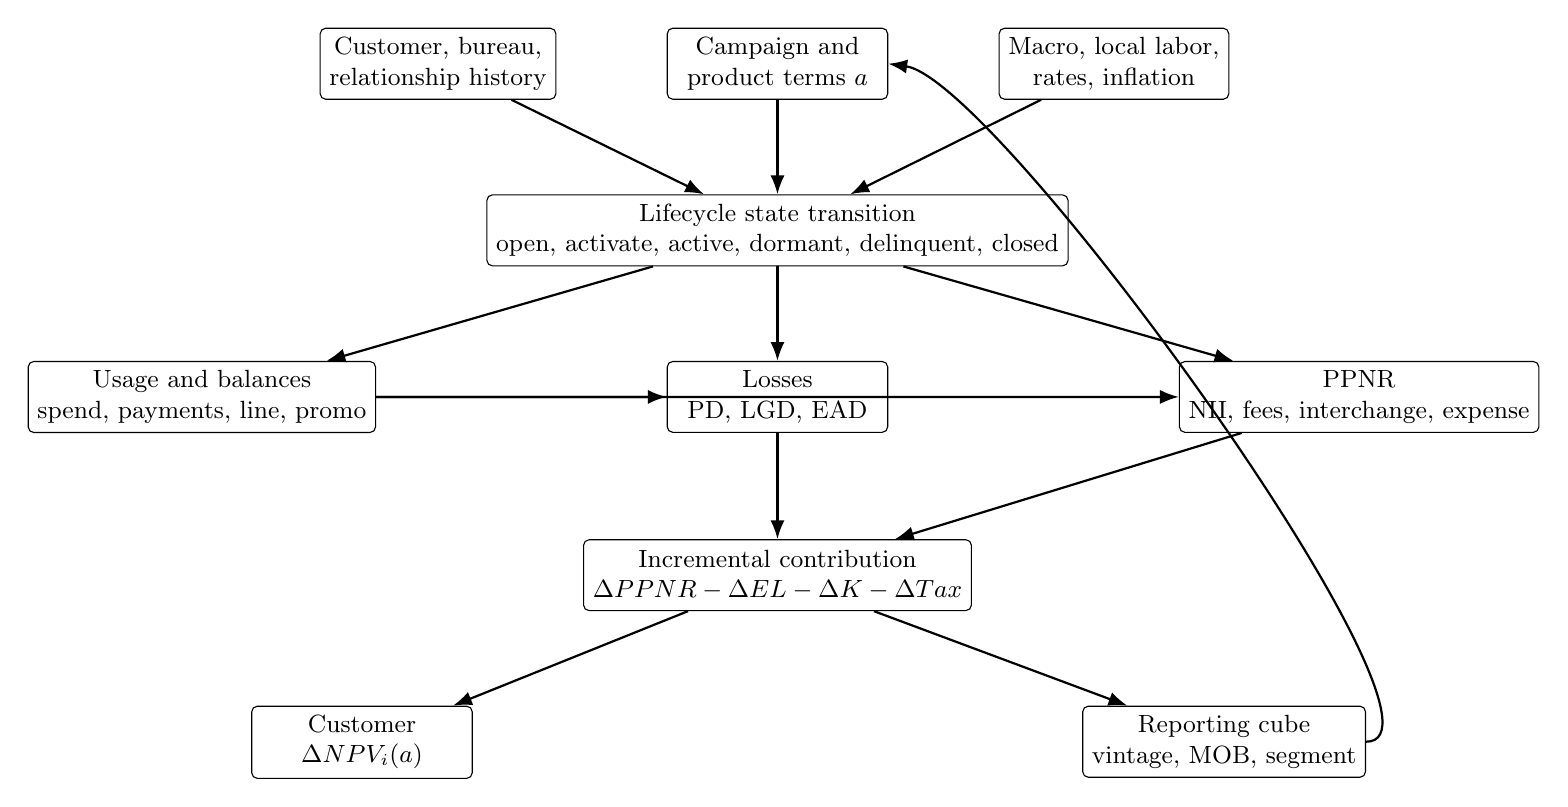
\begin{tikzpicture}[
  node distance=1.2cm and 1.4cm,
  box/.style={
    rectangle,
    draw,
    rounded corners=2pt,
    align=center,
    minimum width=2.8cm,
    minimum height=0.9cm,
    font=\small
  },
  widebox/.style={
    rectangle,
    draw,
    rounded corners=2pt,
    align=center,
    minimum width=4.0cm,
    minimum height=0.9cm,
    font=\small
  },
  arr/.style={-{Latex[length=2.4mm]}, thick}
]
\node[box] (inputs) {Customer, bureau,\\relationship history};
\node[box, right=of inputs] (offer) {Campaign and\\product terms $a$};
\node[box, right=of offer] (macro) {Macro, local labor,\\rates, inflation};

\node[widebox, below=of offer] (state) {Lifecycle state transition\\open, activate, active, dormant, delinquent, closed};

\node[box, below left=of state] (usage) {Usage and balances\\spend, payments, line, promo};
\node[box, below=of state] (loss) {Losses\\PD, LGD, EAD};
\node[box, below right=of state] (ppnr) {PPNR\\NII, fees, interchange, expense};

\node[widebox, below=1.35cm of loss] (finance) {Incremental contribution\\$\Delta PPNR-\Delta EL-\Delta K-\Delta Tax$};
\node[box, below left=of finance] (npv) {Customer\\$\Delta NPV_i(a)$};
\node[box, below right=of finance] (report) {Reporting cube\\vintage, MOB, segment};

\draw[arr] (inputs) -- (state);
\draw[arr] (offer) -- (state);
\draw[arr] (macro) -- (state);
\draw[arr] (state) -- (usage);
\draw[arr] (state) -- (loss);
\draw[arr] (state) -- (ppnr);
\draw[arr] (usage) -- (loss);
\draw[arr] (usage) -- (ppnr);
\draw[arr] (loss) -- (finance);
\draw[arr] (ppnr) -- (finance);
\draw[arr] (finance) -- (npv);
\draw[arr] (finance) -- (report);
\draw[arr] (report.east) .. controls +(1.4,0.0) and +(1.4,-0.2) .. (offer.east);
\end{tikzpicture}%
}
\caption{Schematic architecture for a component-based incremental NPV engine.}
\label{fig:component-system}
\end{figure}

\subsection{Connection Back to Incremental NPV}
\label{subsec:component-to-npv}

The component architecture is useful only if every module feeds the same
counterfactual cash-flow primitive introduced in
Equation~\eqref{eq:incremental-cash-flow}. The final object should be
\begin{align}
  \Delta \NPV_i(a;d,s,\pi)
  &=
  - C_i^{\mathrm{acq}}(a)
  +
  \sum_{h=0}^{H}
  \delta_h\,
  \E\!\left[
    \Delta CF_{i,t+h}(a,\pi;s)
    \mid \mathcal{I}_{id}
  \right]
  +
  \delta_H
  \E\!\left[
    \Delta TV_{i,t+H}(a,\pi;s)
    \mid \mathcal{I}_{id}
  \right],
  \label{eq:component-delta-npv}
\end{align}
where each $\Delta$ is relative to no offer, no conversion, or the relevant
business-as-usual action. The module-level PPNR, expected-loss, capital, tax,
and relationship-value terms enter through $\Delta CF$; acquisition cost and
terminal value are shown separately because they are often governed by
different finance assumptions. Table~\ref{tab:component-to-npv} summarizes the
handoff from each component to Equation~\eqref{eq:component-delta-npv}.

\begin{table}[t]
\centering
\caption{Component outputs required by the incremental NPV model.}
\label{tab:component-to-npv}
\begin{tabular}{p{0.20\linewidth}p{0.32\linewidth}p{0.38\linewidth}}
\toprule
Component & Required output & Connection to NPV \\
\midrule
Response and activation
  & $\Delta\Pr(\mathrm{open})$, $\Delta\Pr(\mathrm{active})$,
    $\Delta\Pr(\mathrm{first\ use})$
  & Gates all future spend, balance, expense, and loss paths. \\
Usage and balances
  & Incremental purchases, cash advances, balance transfers, payments, lines,
    promo balances, and utilization
  & Drives interchange, rewards, finance charges, funding cost, EAD, and
    capital. \\
Losses
  & $\Delta PD$, $\Delta LGD$, $\Delta EAD$, and $\Delta EL$
  & Subtracted from PPNR as expected credit loss; also informs capital and
    downside-risk constraints. \\
PPNR
  & Incremental net interest income, non-interest income, and non-interest
    expense
  & Provides pre-loss contribution before expected loss, capital, tax, and
    relationship spillovers. \\
Attrition and conversion
  & Incremental dormancy, closure, retention, and product-migration paths
  & Determines cash-flow duration and whether value is new, retained, or
    cannibalized from another bank product. \\
Relationship module
  & Incremental deposit margin and other-product contribution
  & Added only when credibly caused by the card action, preferably with
    randomized or quasi-experimental evidence. \\
Reporting segmentation
  & Aggregation by product, vintage, MOB, risk, geography, promo, and balance
    type
  & Supports governance, monitoring, and cost actions; does not by itself
    define the optimization target. \\
\bottomrule
\end{tabular}
\end{table}

This framing also clarifies what should be amended in the original
classification. Losses, balances, and PPNR are essential, but the production
system should explicitly include rewards, interchange, fraud/disputes,
servicing and collections, capital and funding, taxes/accounting, relationship
spillovers, and causal cannibalization. The model should preserve the
principal/non-principal subledger and vintage/months-on-book dimensions because
they affect both economics and governance. Finally, cost-cutting decisions
should be evaluated as actions inside the same NPV system rather than as
external heuristics; an inactive account, a promotional account, or a product
conversion is valuable only to the extent that its incremental discounted
contribution is positive after losses, costs, and cannibalization.

\section{Decision and Measurement Pitfalls in Card NPV}
\label{sec:decision-pitfalls}

Several practical concerns about NPV are legitimate. They are not objections to
using NPV; they are reasons the NPV system must be explicitly staged, causal,
and uncertainty-aware. The marketing and CLV literatures motivate a discounted
contribution objective \citep{bult1995directmail,berger1998clv,rust2004return,venkatesan2004clv},
but the card setting adds long-horizon credit, funding, capital, and account
management dynamics. The right response is not to replace NPV with response,
approval, or sales volume. It is to make clear which NPV is being estimated, for
which decision, on which population, and under which downstream policy.

\subsection{NPV Is a Long-Horizon Latent Quantity}
\label{subsec:npv-latent}

Customer NPV is unintuitive because it is not directly observed. The bank
observes partial cash flows over finite calendar time; it does not observe the
counterfactual no-offer path, the customer's full outside-wallet behavior, or
the terminal value of the relationship. A more honest notation is therefore
\begin{equation}
  \Delta \NPV_i(a;\theta,\pi)
  =
  \sum_{h=0}^{H}
  \delta_h
  \E_\theta[
    \Delta CF_{i,t+h}(a,\pi)
    \mid \mathcal{I}_{it}
  ]
  +
  \delta_H
  \E_\theta[
    \Delta TV_{i,t+H}(a,\pi)
    \mid \mathcal{I}_{it}
  ],
  \label{eq:npv-theta-policy}
\end{equation}
where $\theta$ collects model parameters and scenario assumptions, $\pi$ is the
future account-management policy, $\Delta CF$ is the one-period incremental
cash-flow primitive from Equation~\eqref{eq:incremental-cash-flow}, and
$\Delta TV$ is terminal value. This notation makes the instability visible:
rankings can change when assumptions about spend decay, revolve rate,
attrition, default timing, recovery, funding cost, capital cost, or terminal
value change.

A bank implementation should therefore report not only
$\widehat{\Delta \NPV}_i(a)$, but also a sensitivity or posterior distribution:
\begin{equation}
  \left\{
    \Delta \NPV_i(a;\theta^{(s)},\pi^{(s)})
  \right\}_{s=1}^{S}.
  \label{eq:npv-sensitivity-draws}
\end{equation}
For campaign selection, the robust decision statistic may be expected
incremental NPV, lower-tail NPV, probability of negative NPV, or expected NPV
subject to capital and loss constraints. This is consistent with the stress-test
view that balance, revenue, and loss paths should be evaluated under macro
scenarios \citep{federalreserve2025stressmethodology,federalreserve2026stressmethodology}.
It also prevents proxy metrics such as first-90-day spend from silently becoming
promotion criteria for lifetime value.

\subsection{Card Value Is Behaviorally Heterogeneous}
\label{subsec:behavioral-heterogeneity}

The second issue is that card profitability is not one-dimensional. Two
customers with the same first-month spend can have opposite economics if one is
a low-risk transactor with high interchange and modest rewards cost, while the
other revolves promotional balances, pays slowly, uses cash advances, and later
charges off. The appropriate object is a heterogeneous treatment effect over
the full cash-flow vector:
\begin{equation}
  \tau_{V}(x,a)
  =
  \E[V_i(a)-V_i(0)\mid X_i=x],
  \label{eq:value-cate}
\end{equation}
where $V_i$ is not one outcome but the discounted contribution generated by
spend, balances, payments, losses, rewards, fraud, servicing, funding, and
capital. Uplift and causal-forest methods are useful for estimating
heterogeneous treatment effects \citep{lo2002true,wager2018causalforests,chernozhukov2018dml},
and statistical treatment-rule work emphasizes choosing actions by expected
welfare or payoff under heterogeneity rather than by average effect alone
\citep{manski2004treatment}.

This implies that the model should not rank customers by a single revenue or
risk proxy. A useful diagnostic decomposition is
\begin{align}
  \tau_{V}(x,a)
  &=
  \tau_{\mathrm{interchange}}(x,a)
  + \tau_{\mathrm{finance}}(x,a)
  + \tau_{\mathrm{fees}}(x,a)
  - \tau_{\mathrm{rewards}}(x,a) \nonumber\\
  &\quad
  - \tau_{\mathrm{servicing}}(x,a)
  - \tau_{\mathrm{fraud}}(x,a)
  - \tau_{\mathrm{loss}}(x,a)
  - \tau_{\mathrm{funding/capital}}(x,a).
  \label{eq:value-cate-decomposition}
\end{align}
The decomposition need not be estimated by separate independent models; indeed,
the components are linked through balances and states. But it should be
reported, because a high average NPV segment can hide subsegments whose value
comes from fragile assumptions about revolve, funding, or losses.

\subsection{The Evaluated Population Changes Through the Funnel}
\label{subsec:funnel-population}

The population changes as the customer moves from prospect to applicant to
approved account to booked account to active user. This is a selection problem:
the covariates observed, the eligible action set, and the conditional value
distribution all change after each gate. The sample-selection literature is the
classical warning that outcome models estimated only on selected observations
need not describe the original population \citep{heckman1979selection}. In the
card funnel, the same issue appears in operational form:
\begin{align}
  \mathcal{P}_0 &= \{i:\text{marketable prospects}\},\\
  \mathcal{P}_1 &= \{i\in\mathcal{P}_0:\text{respond or apply}\},\\
  \mathcal{P}_2 &= \{i\in\mathcal{P}_1:\text{approved and line assigned}\},\\
  \mathcal{P}_3 &= \{i\in\mathcal{P}_2:\text{booked and activated}\}.
  \label{eq:funnel-populations}
\end{align}
The right estimand changes with the conditioning set. For example,
\begin{align}
  \tau^{\mathrm{target}}(x)
    &= \E[\NPV_i(\mathrm{contact})-\NPV_i(\mathrm{suppress})
        \mid i\in\mathcal{P}_0,X_i=x],\\
  \tau^{\mathrm{approve}}(x)
    &= \E[\NPV_i(\mathrm{approve})-\NPV_i(\mathrm{decline})
        \mid i\in\mathcal{P}_1,X_i=x],\\
  \tau^{\mathrm{usage}}(x)
    &= \E[\NPV_i(\mathrm{line},\mathrm{terms})-\NPV_i(\mathrm{baseline})
        \mid i\in\mathcal{P}_2,X_i=x].
  \label{eq:funnel-estimands}
\end{align}
These are not interchangeable. A targeting model can use prospect and
relationship data but not application-only variables. An underwriting model can
use application and bureau data that were unavailable at prospect selection.
An active-account management model can use payment, utilization, transaction,
service, and delinquency history that do not exist for non-booked prospects.
Therefore, a bank should maintain separate model cards, validation populations,
and data-availability timestamps for each funnel stage.

\subsection{The Counterfactual and Objective Change by Decision}
\label{subsec:decision-counterfactuals}

The fourth issue is that ``the NPV objective'' is not one universal treatment
contrast. It is a family of decision-specific contrasts. Direct-marketing
selection asks whether contact has positive incremental value net of contact
cost \citep{bult1995directmail}. Portfolio budget allocation asks whether card
marketing beats redeploying the same budget to another product, channel, or
retention program. Underwriting asks whether approval creates value relative to
decline, subject to credit policy, fairness, compliance, and risk appetite.
Line assignment asks which line maximizes value over a feasible menu while
respecting loss and capital constraints. Formally,
\begin{equation}
  a_d^*(x)
  \in
  \arg\max_{a\in\mathcal{A}_d(x)}
  \E[
    U_d\{\Delta \NPV_i(a),Risk_i(a),Cap_i(a),Fair_i(a)\}
    \mid X_i=x,\mathcal{P}_d
  ],
  \label{eq:decision-specific-policy}
\end{equation}
where $d$ indexes the decision stage and $\mathcal{A}_d(x)$ is the feasible
action set at that stage. The utility $U_d$ may be expected NPV for low-risk
targeting, constrained NPV for underwriting, or portfolio NPV subject to budget,
capacity, capital, and fairness constraints.

Table~\ref{tab:decision-estimands} gives the operational version. The main
governance point is that a model validated for one row should not be reused for
another row without re-estimating the counterfactual and checking that the
conditioning population and action set match.

\begin{table}[t]
\centering
\caption{Decision-specific counterfactuals for card NPV.}
\label{tab:decision-estimands}
\begin{tabular}{p{0.17\linewidth}p{0.24\linewidth}p{0.24\linewidth}p{0.21\linewidth}}
\toprule
Decision & Population & Counterfactual & Objective \\
\midrule
Targeting
  & Marketable prospects or existing clients
  & Contact versus suppress
  & Incremental NPV net of campaign cost. \\
Budget allocation
  & Eligible campaign universe
  & Card campaign versus redeploy budget
  & Portfolio NPV per scarce marketing dollar or capacity unit. \\
Underwriting
  & Applicants or responders with application data
  & Approve versus decline, or approve with terms versus decline
  & Risk-adjusted NPV subject to policy and compliance constraints. \\
Line assignment
  & Approved or preapproved accounts
  & Line amount $\ell$ versus alternative line amounts
  & NPV over line menu, accounting for usage, EAD, losses, and capital. \\
Account management
  & Booked accounts
  & Maintain, reprice, retain, convert, line change, or close
  & Forward NPV under updated behavior and risk state. \\
\bottomrule
\end{tabular}
\end{table}

\subsection{Decisions Are Interdependent Over Time}
\label{subsec:interdependent-decisions}

Finally, decisions are interdependent. Acquisition changes the population that
underwriting sees. Underwriting and line assignment change the balance,
utilization, and risk states that account management later sees. Future line,
pricing, collections, retention, or conversion policies change the lifetime
economics assumed at acquisition. The dynamic treatment-regime and Markov
decision-process literatures provide useful language for this problem:
the value of an action depends on the future policy that follows it
\citep{puterman1994mdp,murphy2003dynamic,rust1987replacement}.

A compact representation is
\begin{align}
  Z_{i,t+1} &\sim p_\theta(Z_{i,t+1}\mid Z_{it},X_{it},a_t),\\
  CF_{it}  &= c_\theta(Z_{it},X_{it},a_t),\\
  \pi_t    &: (Z_{it},X_{it}) \mapsto a_t,
  \label{eq:dynamic-policy-system}
\end{align}
with policy value
\begin{equation}
  V^\pi_i(z,x)
  =
  \E_\theta^\pi
  \left[
    \sum_{h=0}^{H}\delta_h CF_{i,t+h}
    + \delta_H TV_{i,t+H}
    \mid Z_{it}=z,X_{it}=x
  \right].
  \label{eq:policy-value}
\end{equation}
The acquisition model should therefore state its assumed downstream policy
$\pi$: for example, line-increase rules, repricing rules, collections policy,
retention offers, dormancy closure, and product-conversion policy. If those
policies change, the upstream acquisition NPV should be recalibrated. This is
especially important for cost-cutting initiatives: closing inactive accounts,
reducing promotional offers, tightening lines, or converting products may
improve near-term expense or losses while reducing the value of cohorts that
were acquired under older assumptions.

The practical recommendation is to treat card NPV as a policy-evaluation
system, not a one-time score. Each major decision should store the population,
available variables, action set, counterfactual, downstream policy assumption,
cash-flow decomposition, and sensitivity range. That metadata is not bureaucracy;
it is what prevents an upstream model from optimizing a downstream world that
the bank no longer operates.

\section{Empirical Design and Validation}
\label{sec:validation}

\subsection{Data requirements}

A bank-grade data set should join campaign exposure, channel, creative, offer
terms, application, underwriting, activation, card transactions, balances,
payments, delinquency, charge-off, recoveries, fraud, disputes, servicing,
relationship products, deposits, payroll indicators, bureau refreshes, and
local macro series. The data should preserve timing. Variables measured after
campaign exposure must not be used as if they were available at targeting time.

For the existing-client new-card problem, the data must also identify
cannibalization. At minimum, the bank should measure whether new-card spend
comes from:
\begin{enumerate}[label=\alph*.]
  \item genuinely incremental customer spend;
  \item spend shifted from a competitor card;
  \item spend shifted from the bank's existing card;
  \item debit or deposit activity shifted onto credit;
  \item temporary promotion-induced spend that decays after the offer.
\end{enumerate}
The first two categories are the cleanest direct sources of new issuing-bank
card value, holding other relationship effects fixed. Debit or deposit
substitution, internal old-card shift, and promotion timing can be positive,
neutral, or negative depending on interchange, rewards, deposit economics,
funding, losses, servicing, and durability.

The data set should also identify the evidence grade for outside-wallet and
spend-source estimates. Directly observed or internally anchored quantities
include old-bank-card spend, new-card spend, bank-observed debit activity,
balance transfers into the new card, payoffs from identified accounts,
card-on-file changes visible to the bank, and post-promo decay on the bank's
own book. Externally benchmarked quantities may use bureau tradeline
attributes, network or merchant aggregates where available, public macro and
credit series, and licensed market data. Model-imputed or scenario-only
outside-wallet quantities should be retained for sensitivity analysis, but they
should not be reported as captured competitor wallet or used as proof of
incremental NPV.

\subsection{Promotion criteria}

The primary promotion criterion should be randomized or credibly
quasi-experimental lift in incremental NPV. Response AUC, approval AUC,
activation lift, first-purchase lift, and first-90-day spend are useful
diagnostics, but they are proxy metrics. They should nominate models for
further testing rather than establish lifetime NPV validity.

Recommended validation splits include:
\begin{itemize}[leftmargin=*]
  \item time-based holdouts for economic drift;
  \item campaign randomized holdouts for treatment effects;
  \item vintage holdouts for lifetime trajectories;
  \item macro-stress backtests around unemployment, rate, and inflation shocks;
  \item segment calibration across score bands, income proxies, geography,
        tenure, relationship depth, channel, and product;
  \item counterfactual cannibalization analysis for existing-client offers;
  \item validation anchors for outside-wallet and movable-wallet estimates,
        including balance-transfer or payoff records, old-card spend decay,
        debit/deposit substitution, card-on-file migration, bureau aggregates
        where available, account-aggregation samples, and post-promotion decay.
\end{itemize}

These validation designs should map directly to component gates. A spend model
that fails macro-drift validation should not be used for scenario-sensitive
campaign ranking. A causal lift model that lacks overlap or holdout evidence
should not be used to claim incremental NPV, even if it predicts responders
well. A booked-account model that uses post-approval payment history should not
be used for prospect targeting. A decomposition that does not reconcile to
finance and risk views should not be used for production ranking until the
assumption difference is explained and approved. An outside-wallet model that
has no validation anchor should not be used for precise dollar capture claims.
A target-population diagnostic should compare prospects, contacted customers,
responders, applicants, approved accounts, booked accounts, activated accounts,
and active incumbents before a model trained on one population is used for
another. These are veto conditions for component use, not academic footnotes.

\section{Identification, Endogeneity, and Data Strategy}
\label{sec:identification-data}

The proposal so far decomposes card value into modules: spend, usage,
balances, payments, losses, PPNR, costs, capital, and relationship effects.
That decomposition is necessary, but it creates a serious identification
problem. Many of the variables that predict NPV are also variables that the
bank controls, targets, or observes only after a selected customer passes
through the funnel. A model can predict observed portfolio outcomes under the
current policy and still be wrong for the decision question, ``what is the
incremental NPV if we take action $a$ instead of baseline action $a_0$?''

The causal-inference literature provides the language for this distinction.
Let $Y_i(a)$ denote the future cash-flow path, or one component of it, that
would occur if customer or account $i$ received action $a$. The component
needs objects such as
\begin{equation}
  \E\!\left[Y_i(a)-Y_i(a_0)\mid X_i, d, s, \pi\right],
  \label{eq:causal-cashflow-object}
\end{equation}
not merely $\E[Y_i\mid T_i=a,X_i]$. The latter is an observed-outcome
prediction under the historical treatment rule. It equals the causal object
only under an identification argument: randomized assignment, conditional
exchangeability with overlap, a valid instrument or encouragement design, a
valid discontinuity, a credible difference-in-differences design, or another
defensible quasi-experiment \citep{rosenbaum1983propensity,
imbensrubin2015causal,angrist2009mostlyharmless,imbenswooldridge2009recent,
hernanrobins2020causal}. For a production NPV component, this is not a
philosophical distinction. It determines whether the output may be used to
rank actions or only to monitor expected outcomes.

\subsection{Where endogeneity enters the card NPV modules}

Endogeneity first appears at marketing selection. Campaigns are usually not
sent randomly. Customers with better scores, deeper relationships, attractive
deposit signals, prior engagement, lower expected loss, or lower contact cost
may be more likely to receive an offer. If the model compares contacted
customers with uncontacted customers without accounting for this assignment
rule, it will credit the campaign for value that was already present. A
response model has the same problem in a different form: responders are not a
random subset of prospects, and their post-response value does not identify the
value of contacting the marginal prospect.

The second problem is funnel selection. The evaluated population changes from
prospect to applicant, applicant to approved account, approved account to
booked account, booked account to activated account, and activated account to
seasoned account. At each stage, variables, available outcomes, and economic
meaning change. A model trained on active accounts conditions on response,
approval, booking, and activation. It may be useful for servicing an active
portfolio, but it does not by itself estimate prospect NPV. The sample-selection
problem described by \citet{heckman1979selection} is therefore not a side
issue; it is central to using the component across the funnel.

The third problem is endogenous product terms. Credit line, APR, promotional
duration, balance-transfer terms, rewards, signup bonus, fee waivers, and
retention offers are assigned by policies that already use risk, expected
profitability, capacity, customer tenure, or channel. Those terms then change
usage, balances, payments, losses, rewards cost, funding cost, and attrition.
Naively regressing NPV on line or APR will often recover a mixture of the
customer selection rule and the causal effect of the term. In particular,
high-line accounts can look safer because the bank gave high lines to safer
customers, while a line increase for a marginal account can still raise EAD,
utilization, and loss.

The fourth problem is simultaneity among balances, payments, utilization, and
losses. Payments reduce balances, balances generate interest and funding cost,
line affects utilization, utilization affects risk scores, delinquency affects
collections treatment, and collections treatment affects recovery and attrition.
Conditioning on variables that lie after the action, such as early utilization
or first-payment behavior, can be appropriate for an account-management
decision made later, but it is leakage for a prospect-targeting or initial-line
decision. Dynamic panel methods such as \citet{arellano1991panel} and
\citet{blundell1998initial} are useful warnings here: lagged outcomes and
unobserved heterogeneity cannot be treated as ordinary controls without
thinking through the data-generating process.

The fifth problem is endogenous attrition, dormancy, and account-management
policy. An account can become inactive because the customer lost interest, the
bank reduced rewards, the line was cut, service quality deteriorated, fraud or
dispute experience changed the relationship, another card became more
attractive, or the customer entered financial distress. Closure, retention,
repricing, hardship, and conversion policies are themselves actions. If the
component estimates lifetime value only among surviving accounts, it builds in
survivorship bias. If it ignores future policy, it values a customer under an
operating regime that may not be the one the bank will actually run.

The sixth problem is macro and geography confounding. Market conditions,
employment, rates, inflation, housing, merchant mix, and local shocks affect
spend, payments, balances, and credit losses. But campaigns and policy changes
also occur in calendar time and may be geographically targeted. A campaign run
in a strong labor market can appear profitable because unemployment was falling,
not because the offer had high incremental value. A line-tightening policy
implemented during a downturn can look harmful or helpful depending on which
macro controls and comparison cohorts are used. This is why the macro
literature in Section~\ref{sec:macro} should be connected to identification,
not used only as a list of predictors.

Finally, relationship value and deposit spillovers are especially vulnerable
to confounding. Customers who take a premium card, keep large deposits, use
digital channels, and buy other products are often already more engaged. The
component should not count deposit growth, brokerage balances, or other-product
profit as card-caused NPV unless there is evidence that the card action changed
the relationship. Without that evidence, relationship value should be reported
as an associated outcome or scenario sensitivity, not added silently to
incremental card NPV.

\subsection{Identification designs for component modules}

The strongest design is randomized treatment assignment with a preserved
control group. For marketing and cross-sell, this means campaign holdouts,
channel holdouts, offer-cell randomization, and, where feasible, randomization
over creative, rewards, promo duration, or line invitation. The component
should treat those experiments as first-class data assets. It should ingest the
randomization unit, assignment probability, treatment arm, eligibility rule,
holdout flag, campaign calendar, and offer terms. When a randomized design is
valid and sufficiently powered, the treatment effect can be estimated directly
or with covariate adjustment, and heterogeneous treatment-effect methods can be
used to learn which customers have positive incremental NPV.

Randomization is not always feasible. Encouragement designs can still help
when the bank can randomize an invitation, reminder, channel placement, or
prequalified offer while the final take-up decision remains voluntary. The
instrumental-variables literature, especially the local-average-treatment-effect
framework of \citet{angristimbensrubin1996iv}, is relevant because the effect
is identified for customers whose treatment status is changed by the
encouragement, not for every customer. The NPV component should therefore label
such estimates as complier effects and should not extrapolate them to customers
with very different take-up behavior without a separate model-risk approval.

When assignment is observational but rich pre-treatment data are available,
propensity-score and doubly robust methods are useful starting points
\citep{rosenbaum1983propensity,imbenswooldridge2009recent}. The required
component discipline is pre-treatment feature construction, overlap checking,
balance diagnostics, and explicit logging of the estimand. Doubly robust or
double/debiased machine-learning estimators can reduce sensitivity to flexible
nuisance models \citep{chernozhukov2018dml}, and causal forests can estimate
heterogeneous effects \citep{wager2018causalforests}. These methods do not make
selection vanish. They require that the variables sufficient to make treatment
as-good-as-random are observed, measured before treatment, and available for
both treated and control populations.

Regression-discontinuity designs can be useful around score cutoffs, credit
policy thresholds, line-assignment bands, prescreen eligibility thresholds, or
pricing tiers \citep{lee2010rd}. The strength of the design is local
comparison near a threshold; the weakness is that the effect may not generalize
far from that threshold. If the component uses such evidence, the response
should state the threshold, bandwidth, population, and extrapolation status.
For line assignment, this is often a better design than comparing all high-line
and low-line accounts.

Difference-in-differences and event-study designs can be useful for policy
changes, rewards changes, pricing changes, market shocks, or state-level
implementation differences. They require a credible comparison group and
pre-trend evidence. Modern difference-in-differences work shows that staggered
treatment timing and heterogeneous effects can make naive two-way fixed-effect
event studies misleading \citep{callaway2021did,sun2021eventstudy}. The
component should therefore record the cohort timing, comparison population,
pre-trend diagnostics, and estimator class. A failed pre-trend or placebo test
should downgrade the estimate to diagnostic status.

For outcomes observed only after selection, the component should separate the
selection equation from the outcome equation. A prospect-level model may need
application probability, approval probability, booking probability, activation
probability, and conditional lifetime value as separate components. Selection
corrections in the spirit of \citet{heckman1979selection} can be useful when
there is a defensible exclusion restriction. More often, the practical remedy
is data preservation: keep suppressed prospects, nonresponders, applicants,
declines, approvals, bookings, inactive accounts, closures, and charge-offs in
the analytic base, with the decision-time information available at each stage.

For sequential account-management decisions, static treatment effects are not
enough. A card acquired today may later receive line increases, repricing,
retention offers, hardship treatment, collections treatment, or product
conversion. Dynamic treatment-regime and Markov decision-process literature
\citep{murphy2003dynamic,puterman1994mdp} supports the requirement that the
component tag the downstream policy bundle used in valuation. If the bank
changes the downstream policy, the acquisition NPV should not be assumed
unchanged.

The result is a hierarchy of evidence for NPV use. Randomized experiments with
preserved controls should support production treatment ranking when finance
and risk reconciliation also pass. Credible quasi-experiments can support
bounded production use within the identified population. Observational
adjustment can support challenger models, monitoring, and carefully governed
use when overlap and balance diagnostics are strong. Pure prediction should be
used for expected outcome forecasting under current policy, not for causal
claims about alternative actions.

\subsection{Public and licensed external data}

External data are valuable, but they should be used for the right job. They
support scenario construction, macro controls, benchmarking, vintage context,
competitive context, and prior distributions. They generally do not identify
the customer-level causal effect of this bank's card offer, line amount, APR,
reward, or retention action. The proposal should state that boundary clearly.

Federal Reserve Enhanced Financial Accounts and Distributional Financial
Accounts are useful for household balance-sheet context, distributional wealth
and debt aggregates, and macro-financial scenario priors
\citep{federalreserveEFA}. They can help segment a scenario by household
balance-sheet vulnerability or validate whether aggregate portfolio behavior is
plausible. They do not reveal how a particular customer would have spent on
this bank's new card under a randomized offer.

Federal Reserve G.19 consumer-credit data provide aggregate revolving and
nonrevolving consumer-credit context \citep{federalreserveG19}. Z.1 Financial
Accounts provide broader household and financial-sector balance-sheet context
\citep{federalreserveZ1}. These series are useful for macro controls, scenario
alignment, portfolio benchmarking, and explaining whether a backtest period was
credit-expansionary or credit-contractionary.

The New York Fed Household Debt and Credit Report and the underlying Consumer
Credit Panel ecosystem provide benchmark information on balances, delinquency,
credit-card debt, and consumer-credit transitions at aggregate and segmented
levels \citep{nyfedHhdc}. The useful role for the NPV component is external
benchmarking of delinquency, credit-card balance, and transition assumptions,
especially by vintage, age, score band, or geography where public cuts are
available. The role is not replacement of issuer-level PD, LGD, EAD, or
activation calibration.

Labor-market and regional-economic data should feed the spend, payment, and
loss modules as scenario and control variables. BLS Local Area Unemployment
Statistics can provide local unemployment and labor-force measures
\citep{blsLAUS}. BEA regional accounts can provide state and local personal
income, GDP, and related regional indicators \citep{beaRegional}. Census ACS
can provide demographic, income, housing, commuting, and household composition
controls at aggregate geographies \citep{censusACS}. These data are useful for
macro and geography controls, segmentation, monitoring, and fairness-risk
review subject to legal and compliance governance. They should be joined using
approved geography and time keys, not used to infer prohibited characteristics
or make unsupported individual causal claims.

CFPB public credit-card data, including card agreements, terms surveys, and
related public consumer-finance information, can help benchmark product terms,
fees, APR structures, and market practices \citep{cfpbCreditCardData}. These
sources are useful for competitive and policy context, especially when the
component compares offer terms or explains why rewards, fees, and disclosure
changes should be explicit. They are not a substitute for the bank's own reward
cost, activation, revolve, loss, and attrition experience.

FRED and ALFRED are useful data-delivery and vintage-control sources
\citep{fredALFRED}. ALFRED-style real-time vintages matter because a backtest
that uses revised unemployment, income, inflation, or rate data can overstate
the information the bank actually had at campaign or line-decision time. The
NPV component should preserve both the event date and the macro-data vintage
used in training and scoring.

Because the bank has a Refinitiv/LSEG license, the component team should also
inventory entitled LSEG Workspace and economic-data feeds
\citep{lsegWorkspace,lsegEconomicData}. Depending on entitlement, useful
categories may include rates and yield curves, inflation and macro series,
market-implied recession or credit-risk indicators, consumer-sector equity and
earnings data, issuer and competitor financials, credit spreads, asset-backed
securities market indicators, and merchant or sector indicators. These feeds
can improve funding-cost curves, discounting, stress scenarios, competitive
context, and early-warning monitoring. The proposal should not assume that any
particular proprietary field is licensed or approved for model use until data
governance confirms entitlement, permitted use, lineage, retention, and
redistribution limits.

\subsection{Internal data and selection-safe construction}

The bank's internal data are the only plausible source for issuer-specific
activation, usage, cannibalization, loss response, reward cost, servicing cost,
and relationship spillover. The component should therefore require an analytic
base table that preserves the funnel rather than only the booked portfolio. At
minimum, it should include campaign eligibility, suppression rules, contact
assignment, randomization and holdout flags, channel, creative, offer terms,
prescreen variables, application data, approval, decline, refer, override,
booking, activation, transaction, balance, payment, delinquency, charge-off,
recovery, fraud, dispute, servicing, complaints, rewards, account-management
treatments, deposits, payroll indicators, relationship products, bureau
refreshes, and local macro joins.

The most important engineering requirement is time. Each row used for
training or scoring should have an as-of timestamp, decision timestamp,
feature-cut timestamp, outcome window, treatment timestamp, macro-data vintage,
and policy-bundle identifier. Variables created after treatment should be
available only for later decisions. For example, first-purchase behavior can
help value a retention offer after activation, but it cannot be used to decide
whether to target the prospect before the card is opened. This feature-cut rule
is the practical defense against post-treatment leakage.

For existing-client cross-sell, the internal data should preserve all-bank
spend, old-card spend, new-card spend, debit activity, deposit flows, merchant
category, digital-wallet provisioning, autopay, promotional balances,
balance-transfer activity, cash advances, and reward-redemption behavior. The
component should estimate not only new-card spend but all-bank incremental
value. If the bank cannot observe competitor-card spend, the proposal should
state the missing counterfactual and use experiments, bureau aggregates where
available, or sensitivity bounds rather than pretending the outside-card
counterfactual is observed.

For losses, internal data must connect underwriting, line assignment,
utilization, delinquency, collections, charge-off, recovery, hardship,
bankruptcy, and account closure. PD, LGD, and EAD should be estimated on
decision-appropriate populations. A booked-account PD model can support booked
portfolio forecasting; prospect-level expected loss additionally needs
application, approval, booking, and activation selection. Principal and
non-principal balances, promotional balances, fees, accrued interest, cash
advances, and balance transfers should be kept separate because they have
different revenue, loss, payment, and accounting behavior.

For PPNR and costs, internal finance data should provide rewards expense,
interchange, fees, interest income, charge reversals, fraud expense,
collections cost, servicing cost, dispute cost, acquisition cost, funding
transfer pricing, capital charge, tax convention, and allocated overhead. The
component should reconcile behavioral forecasts to finance definitions, but it
should not become the official ledger. Differences between model cash flows and
finance reporting should be explained through valuation-semantics identifiers
and reconciliation reports.

The component should also preserve decision logs from current systems. The
historical policy that generated treatment assignment is itself data. Marketing
scores, eligibility rules, prescreen criteria, underwriting score cutoffs,
manual overrides, line caps, APR matrices, channel capacity, budget constraints,
collection queues, retention rules, and closure rules help explain why a
customer received an action. Without those logs, observational adjustment is
often weak because the most important confounder is the bank's own prior view
of the customer.

\subsection{Estimation ledgers and evidence grades}

The replacement component should maintain estimation ledgers that match the
objects it claims to estimate. These ledgers are not separate governance
paperwork; they are the way the component prevents outside wallet, movable
wallet, causal response, and NPV from being collapsed into one opaque score.

The selection and funnel ledger should compare suppressed prospects,
contacted prospects, responders, applicants, declined applications, approvals,
booked accounts, activated accounts, dormant accounts, and active incumbents.
It should record target-population weights, overlap diagnostics, and segment
calibration. If the model is trained on booked or active accounts but used on
prospects, the response should expose that transportability status.

The offer and terms ledger should record contact channel, creative, reward,
signup bonus, annual fee, APR, balance-transfer terms, promotional duration,
line, fee waivers, repricing, retention treatment, eligibility rule, and any
manual or policy override. It should also record whether each term was
randomized, policy-driven, negotiated, manually overridden, or imputed. This
ledger is essential because line, APR, rewards, and promotions are bank
actions, not passive covariates.

The outside-wallet and cannibalization ledger should record the source of each
outside spend, outside balance, movable-wallet, and spend-source estimate:
directly observed, internally anchored, externally benchmarked,
experimentally identified, quasi-experimental, model-imputed, or scenario-only.
It should also record the uncertainty interval and any cap or reconciliation
constraint, such as estimated moved spend not exceeding plausible outside
eligible spend.

The dynamic behavior ledger should decompose observed changes into total spend
or borrowing growth, share movement to the bank, internal cannibalization,
debit or deposit substitution, promotion timing, balance build, payment
response, runoff, and attrition. This ledger should be validated out of time,
by vintage, and by stress or macro regime.

The causal evidence ledger should record the experiment, holdout,
encouragement, cutoff, policy change, or observational adjustment supporting
each treatment-response estimate. It should include overlap, balance,
pre-trend, placebo, effective-sample-size, and sensitivity diagnostics. If the
evidence is only associational, the output should be labeled as predictive or
diagnostic, not causal incremental NPV.

The downstream-policy ledger should record the assumed future line,
repricing, retention, collections, closure, hardship, and product-conversion
policies. A customer acquired under one assumed future policy can have a
different value under another. The NPV output should therefore carry the policy
bundle identifier and should be revalidated when that bundle changes.

\subsection{Production implications for the NPV component}

The identification strategy should be visible in the component contract. Each
NPV response should carry an identification design identifier, population
stage, decision context, treatment definition, baseline definition, feature-cut
timestamp, macro-data vintage, downstream-policy bundle, experiment or holdout
identifier when available, overlap or support score, causal-evidence level,
outside-wallet evidence grade, movable-wallet evidence grade, cannibalization
evidence grade, target-population diagnostic, and allowed-use status. This
metadata is not decoration. It tells the caller whether the number is an
incremental value estimate, an expected-outcome forecast, a scenario diagnostic,
or an extrapolation requiring approval.

The component should implement veto diagnostics. It should warn or refuse
production action-ranking use when treatment-control overlap is poor, balance
diagnostics fail, randomization is broken, pre-trends fail, placebo effects are
large, post-treatment leakage is detected, the model is trained on booked or
active accounts but called for prospects, macro variables use revised rather
than as-of vintages, the caller asks for a decision outside the approved
population, CATE estimates are unstable, or finance/risk reconciliation fails.
The component should also warn when estimated moved wallet exceeds plausible
outside wallet, when temporary promotion lift is being used as durable wallet
share, or when a model-imputed outside-wallet value is being used as if it were
directly observed or experimentally identified. These gates are how the
literature becomes an operating control.

The component should also distinguish three output classes. First,
\emph{causal incremental NPV} is supported by randomized or credible
quasi-experimental evidence and may be used for governed action ranking within
the approved population. Second, \emph{policy-conditional expected NPV}
predicts outcomes under the historical or declared policy and may be used for
planning, monitoring, and portfolio forecasting, but not as proof that a
different action would create value. Third, \emph{diagnostic or benchmark NPV}
uses external data, weak observational evidence, or scenario assumptions and
should be labeled for sensitivity analysis or management review. A single
scalar without this class label is not an acceptable replacement component.

These requirements should be part of the replacement component package. Each
module should have an identification note, a data-lineage specification, an
experiment and holdout inventory, a decision-stage analytic-base design, a
leakage-control checklist, a public and licensed data inventory, and a
validation gate that separates predictive accuracy from causal incremental
value. These artifacts determine which submodel outputs can enter
Equation~\eqref{eq:proposal-objective} for each caller and which outputs must
remain warnings, diagnostics, or assumptions.

\section{Open Gaps and Reviewer Risks}

The public literature does not fully identify issuer-specific new-card usage
and incremental NPV. Payment-choice and rewards studies show mechanisms, but
the activation probability for a particular bank, product, offer, channel, and
customer segment is a proprietary empirical object. Likewise, CLV models provide
powerful baselines for transaction frequency and duration, but bank NPV requires
integration with expected credit loss, rewards, fraud, funding, capital, and
regulatory constraints.

The largest reviewer risks are:
\begin{enumerate}[label=\arabic*.]
  \item treating activation or first spend as lifetime NPV evidence;
  \item treating raw propensity as causal lift;
  \item ignoring cannibalization from the bank's existing cards;
  \item estimating spend without macro and employment state dependence;
  \item separating marketing CLV from credit risk and balance-sheet cost;
  \item using public rewards estimates as universal program parameters;
  \item reusing one NPV model across targeting, underwriting, line assignment,
        and account management without changing the counterfactual;
  \item validating on booked or active accounts while applying the result to
        prospects or applicants without correcting for funnel selection;
  \item treating product terms such as line, APR, promo duration, rewards, or
        fee waiver as exogenous predictors when they were assigned by bank
        policy;
  \item using public macro, credit, or market data as if they identify
        customer-level treatment effects rather than scenario, control,
        benchmark, or prior information;
  \item adding deposit, relationship, or other-product value to card NPV
        without evidence that the card action caused the relationship change;
  \item treating observed new-card spend as captured outside wallet;
  \item treating estimated outside wallet as offer-specific movable wallet;
  \item treating wallet size or movable-wallet size as NPV before rewards,
        losses, funding, capital, fraud, servicing, and attrition are netted;
  \item using model-imputed wallet estimates as if they were directly observed
        or experimentally identified;
  \item treating temporary promotion lift as durable wallet-share capture.
\end{enumerate}

\section{Alternatives and Tradeoffs}
\label{sec:alternatives-tradeoffs}

Several simpler approaches are possible, and each is useful for a limited
purpose. The reason for recommending a modular NPV component is not that these
alternatives are worthless. It is that none of them is sufficient as the
replacement valuation component for a large bank once the decision spans
marketing, new-card cross-sell, line assignment, offer design, account
management, finance reconciliation, and model-risk review.

A response or propensity model is the natural first alternative. It is fast to
build, easy to monitor, and operationally familiar. It can improve campaign
execution by estimating who is likely to respond, apply, activate, or make a
first purchase. The direct-marketing literature, however, already warns against
optimizing response alone: the decision should depend on expected net return,
not merely on response probability \citep{bult1995directmail}. In a card
portfolio, this limitation is sharper because response does not price rewards,
losses, funding, capital, servicing, fraud, attrition, or cannibalized spend.
Propensity models should therefore remain funnel modules and diagnostics, not
the final value object.

A second alternative is a standard CLV model with a finance overlay. This is
closer to the economic target because CLV explicitly discounts future
contribution and has mature models for purchase frequency, duration, and
retention \citep{berger1998clv,rust2004return,venkatesan2004clv,
schmittlein1987counting,fader2005bgnbd}. It is a useful baseline for lifetime
activity. The tradeoff is that plain CLV does not by itself solve the card
problems that matter most for bank use: PD, LGD, EAD, line and APR policy,
principal versus non-principal balances, rewards liability, funding transfer
pricing, capital charges, and within-bank cannibalization. A finance overlay
can patch some of these terms, but if the overlay is added after behavior is
forecast, it can miss the fact that product terms and account-management
policies change behavior itself.

A third alternative is to rely on randomized holdouts and causal lift studies
without a full dynamic NPV engine. This is attractive because experiments are
the cleanest evidence for incremental value, and the proposal should treat
campaign holdouts and offer-cell randomization as first-class assets. The
limitation is horizon and policy dependence. A campaign experiment may
identify 90-day activation, spend lift, or early loss differences, but it does
not automatically identify five-year value under future line increases,
repricing, retention offers, collections policies, macro shocks, and terminal
value assumptions. Experiments should anchor the causal layer; they do not
remove the need for a governed forecast and valuation layer.

A fourth alternative is a monolithic machine-learning value score trained on
historical realized profitability. This can produce a strong offline fit and
may be useful as a challenger benchmark. It is risky as the production
replacement if it hides the target population, treatment assignment, feature
timing, finance definitions, and decomposition. A model trained on booked or
active accounts can look accurate while being invalid for prospects. A score
that uses post-treatment features can leak future information. A realized
profitability target can combine organic customer quality with the effect of
the bank action. These are not cosmetic model-risk issues; they change the
counterfactual being estimated.

The recommended architecture is therefore a modular NPV component with clear
valuation semantics. It uses response, activation, CLV, credit-risk, PPNR,
capital, cost, and causal-lift models, but it does not collapse them into an
uninterpreted scalar. Its cost is additional data lineage, governance, and
reconciliation work. Its benefit is that a reviewer can inspect why a customer
is valuable, whether the value is causal or predictive, which population the
evidence supports, how losses and capital enter, and what assumptions would
change the ranking. The practical rollout should still be phased: start with a
controlled batch acquisition or prescreen slice, retain simpler models as
baselines and diagnostics, and expand use cases only when the component-level
evidence and integration contracts support them.

\section{Using the Component in Existing Bank Decision Processes}
\label{sec:decision-use}

The component should be used only through an explicit decision-context
contract. That contract is simple in concept even if the implementation schema
is detailed. The caller must say who or what is being scored, which decision is
being valued, what action alternatives are feasible, what baseline defines the
counterfactual, what information was available at the decision time, what
valuation semantics and scenario are being used, and what downstream policy is
assumed. The component then returns a decomposed value object, status, warning
set, and lineage. The caller remains responsible for action choice and
execution.

The most important use cases are different enough that they should not share
one generic interpretation of NPV. For new-to-bank targeting, the baseline is
usually suppress and the action is contact through a channel and offer. For
existing-client new-card cross-sell, the baseline is no new-card offer and the
central risk is cannibalizing existing bank-card or debit activity. For
underwriting, the baseline is decline or refer and the action must remain
inside approved credit policy. For line assignment, the component values a
menu of feasible line or term options and must expose usage, EAD, loss, and
capital for each option. For retention, inactivity, product conversion, and
promotional treatment, the baseline is the organic account path and the action
may change attrition, rewards, servicing, balances, and losses.

Valuation semantics must be visible for every use. A value number should not
move through the bank unless its horizon, discounting, funding, capital, tax,
cost allocation, rewards, relationship value, cannibalization, terminal value,
scenario, and downstream-policy assumptions are tagged. This is not a
technical nicety. Without the tag, two callers can compare numbers that are
both called NPV but are economically different.

The response should be decomposed enough to diagnose why a customer or option
is valuable. A high expected value from interchange is different from a high
expected value from revolve. A high value dominated by terminal value is
different from one dominated by near-term spend. A positive new-card-spend
lift with near-zero all-bank-spend lift is a cannibalization warning, not a
success. A high-line option with higher spend but materially higher EAD and
capital should not be treated as a pure revenue win. These distinctions are
why the component must return paths, decomposition, uncertainty, and status,
not only a scalar.

Status semantics protect callers from silent misuse. A no-score because the
use case is unapproved is different from a technical timeout. A degraded score
because merchant-category history is missing is different from an
out-of-domain population. A batch job can succeed while individual rows fail;
an option grid can score one line amount while rejecting another. Those states
should be explicit in the response and preserved for replay.

\section{Migration, Governance, and First Production Slice}
\label{sec:main-governance-migration}

The replacement should be introduced as a controlled component migration, not
as a one-time model launch. The first production slice should remain narrow:
one batch acquisition or prescreen consumer, one offer family, one valuation
semantics bundle, frozen feature snapshots, campaign holdouts, and shadow
scoring against the current component. This slice is valuable because it
exercises the full NPV chain without adding real-time underwriting or
account-management risk.

Migration should begin by inventorying the current component. The bank needs
to know every consumer, field, threshold, fallback, owner, latency class,
report, and downstream decision that currently depends on the old value. It
then needs a valuation-definition comparison: horizon, discounting, funding,
capital, tax, cost, reward, terminal value, scenario, and policy assumptions
in the old component versus the new one. Without this comparison, a ranking
change can look like a model improvement when it is actually an assumption
change.

Shadow scoring should compare both values and decisions. The bank should
measure rank correlation, top-decile overlap, segment-level aggregate NPV,
component decomposition tie-outs, no-score and degraded-score rates,
disagreement patterns, and downstream contract behavior. Material
disagreements should be put in a register and classified as expected
improvements, assumption differences, data issues, unsupported use cases, or
blockers. Cutover should occur by controlled consumer and decision context,
not globally.

Governance should separate five questions. Does the model predict the
behavioral paths it claims to predict? Does it estimate causal lift for actions
that change outcomes? Does the decomposition reconcile to finance, treasury,
risk, and product definitions? Do the data and integration pipelines preserve
as-of timing, schema stability, replay, and status semantics? Is the proposed
use case approved by business, model risk, compliance, legal, and technology
owners where required? A positive answer for marketing targeting does not
approve underwriting, line assignment, account closure, collections, adverse
action, CECL, stress testing, or official finance reporting.

Rollback should be designed before launch. Trigger examples include schema
breaks, no-score or degraded-score rates above threshold, failed finance or
risk tie-out, material unexplained ranking movement, replay failure, feature
leakage, out-of-domain drift, or use outside the approved decision context.
Rollback may mean returning to the legacy component, suppressing a campaign,
using a conservative no-score policy, or routing to manual review, depending
on the consumer and use case.

\section{Conclusion}
\label{sec:conclusion}

The replacement component should estimate incremental, risk-adjusted customer
NPV, not response, approval, activation, or new-card spend alone. The
literature supports the mechanisms that make this necessary: market
conditions, employment, liquidity, credit terms, rewards, adoption, and
customer duration affect spend, balances, payments, attrition, and losses. The
literature does not supply this bank's activation rate, cannibalization rate,
movable-wallet share, loss elasticity, funding cost, capital charge, or
relationship spillover. Those are issuer-specific empirical quantities that
must be estimated from the bank's own experiments, quasi-experiments, internal
data, external benchmarks, and finance/risk reconciliations.

The proposal therefore recommends a modular valuation component with explicit
decision context, valuation semantics, scenario, downstream-policy assumption,
decomposition, status, lineage, and allowed-use metadata. The first slice
should be a controlled batch acquisition or prescreen use case, with holdouts,
shadow scoring, reconciliation against the current component, and governed
cutover. Broader use in underwriting, line assignment, existing-account
treatment, finance planning, or account management should be approved only
after the relevant counterfactual, population, data lineage, and validation
evidence support that use.

\appendix

\section{Reference Operating Specification for the Replacement NPV Component}
\label{sec:operating-spec}

The preceding sections establish what the component must estimate and why.
This section translates those requirements into the contract by which existing
bank systems call the replacement component. These contracts are not generic
platform design. They are controls against the exact failure modes identified
above: NPV is latent, value is heterogeneous, populations change through the
funnel, counterfactuals differ by decision, and downstream policies change
upstream economics. The purpose is to make the NPV component replaceable,
testable, auditable, and useful across many callers without letting one
ambiguous value field leak into incompatible decisions.

The operating specification therefore has a narrow job. It tells each caller
how to declare the decision context, baseline, feasible action set, feature
stage, scenario, valuation semantics, and downstream policy assumption. It
tells the component how to return value, decomposition, sensitivity, warnings,
status, and lineage. It does not tell marketing which customers to contact,
underwriting which applications to approve, account management which treatment
to execute, or finance which official ledger number to book.

\subsection{Decision-context contract}
\label{subsec:decision-context-contract}

Every request must declare the decision context, baseline action, candidate
action or option grid, population, feature stage, scenario, valuation semantics,
and downstream policy assumption. This is not administrative ornament. It is
the only way to prevent a value model validated for contact-versus-suppress
from being reused for approve-versus-decline, line assignment, or account
closure.

The component should support at least three groups of consumers.

\paragraph{Acquisition and new-card cross-sell.}
These calls occur before the account is booked or before a new product is
accepted. The available features may be prospect-level, prescreen-level,
relationship-level, or application-level. The primary risk is using
post-decision data or mistaking new-card spend for incremental all-bank value.

\begin{longtable}{L{0.15\linewidth}L{0.14\linewidth}L{0.14\linewidth}L{0.20\linewidth}L{0.23\linewidth}}
\caption{Decision-context contract for acquisition and new-card cross-sell.}
\label{tab:acq-contract}\\
\toprule
Context & Caller & Scored unit & Baseline and action set & Required output \\
\midrule
\endfirsthead
\toprule
Context & Caller & Scored unit & Baseline and action set & Required output \\
\midrule
\endhead
New-to-bank targeting
  & Marketing platform
  & Prospect or household
  & Suppress versus contact through one or more channels/offers
  & Incremental NPV net of contact and acquisition cost; caller owns campaign
    execution. \\
Existing-client new-card cross-sell
  & CRM or cross-sell system
  & Customer, household, or relationship
  & No new-card offer versus offer menu
  & Incremental all-bank value after cannibalization, plus diagnostic new-card
    spend; caller owns offer execution. \\
Prescreen or preapproval
  & Prescreen system
  & Prospect or existing client
  & No prescreen versus preapproved offer terms
  & Expected value conditional on prescreen eligibility, response, approval,
    and booked account economics. \\
Application underwriting
  & Underwriting engine
  & Application
  & Decline, refer, or approve with feasible terms
  & Risk-adjusted value under approved credit policy; underwriting owns final
    decision and compliance process. \\
Initial line and offer assignment
  & Line or offer engine
  & Approved application or account-action pair
  & Feasible line/terms menu
  & Option-level NPV, usage, EAD, loss, capital, and sensitivity paths; caller
    owns chosen line. \\
\bottomrule
\end{longtable}

\paragraph{Existing-account treatment.}
These calls occur after an account exists. The component may use payment,
transaction, utilization, delinquency, service, dispute, rewards, and dormancy
history that is unavailable earlier in the funnel. That means validation on
active accounts cannot be back-projected to prospects without a separate
selection argument.

\begin{longtable}{L{0.16\linewidth}L{0.16\linewidth}L{0.17\linewidth}L{0.18\linewidth}L{0.19\linewidth}}
\caption{Decision-context contract for existing-account treatment.}
\label{tab:acct-contract}\\
\toprule
Context & Caller & Scored unit & Baseline and action set & Required output \\
\midrule
\endfirsthead
\toprule
Context & Caller & Scored unit & Baseline and action set & Required output \\
\midrule
\endhead
Line increase or decrease
  & Account-management or line engine
  & Account-action pair
  & Current line versus feasible line menu
  & Forward NPV, utilization, EAD, PD, LGD, capital, and attrition effects. \\
Retention or inactivity treatment
  & Retention or servicing system
  & Account or relationship
  & No treatment versus fee waiver, reward, line, closure, or contact option
  & Incremental retained value net of concession, servicing, and adverse
    selection. \\
Product conversion
  & Product or CRM system
  & Account-product pair
  & Organic path versus conversion menu
  & Incremental value after annual fee, rewards, cannibalization, attrition,
    and customer-state transitions. \\
Promotional balance or reward treatment
  & Offer or balance-transfer engine
  & Account-action pair
  & No promotion versus promo terms
  & Promo-state NPV, reward liability, funding, post-promo attrition, and loss
    path. \\
Collections-sensitive forward value
  & Servicing or collections system where permitted
  & Account
  & Current treatment path versus approved alternatives
  & Forward value under hardship, collections, recovery, and compliance
    constraints; caller owns customer treatment. \\
\bottomrule
\end{longtable}

\paragraph{Offline finance, risk, and portfolio consumers.}
Offline consumers should use component outputs for analysis and reconciliation,
not as evidence that the NPV component owns finance reporting, CECL, stress
testing, or enterprise dashboards.

\begin{longtable}{L{0.18\linewidth}L{0.18\linewidth}L{0.22\linewidth}L{0.32\linewidth}}
\caption{Offline consumers of component output.}
\label{tab:offline-contract}\\
\toprule
Use & Consumer & Scored unit & Boundary \\
\midrule
\endfirsthead
\toprule
Use & Consumer & Scored unit & Boundary \\
\midrule
\endhead
Campaign budget analytics
  & Marketing analytics
  & Portfolio or campaign universe
  & Component supplies value and drivers; budget optimizer remains outside
    scope. \\
Vintage profitability review
  & Product, finance, and risk
  & Vintage, campaign, product, or segment
  & Component supplies decomposed values; official finance reporting remains
    outside scope. \\
Scenario and planning analysis
  & Finance, treasury, risk, planning
  & Portfolio and segment
  & Component can evaluate approved scenario bundles; stress and planning
    platforms remain outside scope. \\
Model-risk review and monitoring
  & Model-risk management
  & Use case, model version, segment
  & Component supplies lineage, validation, drift, and reconciliation artifacts;
    model-risk approval remains separate. \\
\bottomrule
\end{longtable}

\subsection{Valuation semantics and assumption contract}
\label{subsec:valuation-semantics}

NPV is a valuation convention, not a natural constant. Two systems can both
claim to use NPV while differing in horizon, terminal value, discount curve,
funds-transfer pricing, capital charge, tax treatment, reward liability, cost
allocation, relationship value, cannibalization, macro scenario, and downstream
policy. Therefore each request and response should carry a canonical
\code{valuation_semantics_id}. That identifier should resolve to a controlled
assumption bundle with an owner, approval record, effective date, and version.

\begin{longtable}{L{0.19\linewidth}L{0.25\linewidth}L{0.20\linewidth}L{0.26\linewidth}}
\caption{Valuation semantics required for a decision-grade NPV output.}
\label{tab:valuation-semantics}\\
\toprule
Choice & Required definition & Primary approver & Risk if unspecified \\
\midrule
\endfirsthead
\toprule
Choice & Required definition & Primary approver & Risk if unspecified \\
\midrule
\endhead
Value basis
  & Incremental versus total value; pre-tax versus post-tax value
  & Finance and product
  & Callers compare incompatible scores. \\
Horizon and terminal value
  & Explicit horizon, terminal-value formula, and decay assumptions
  & Finance, product, model risk
  & Rankings become dominated by hidden long-horizon assumptions. \\
Discounting and funding
  & Discount curve, funds-transfer-pricing curve, liquidity basis
  & Treasury and finance
  & Balance-heavy accounts are over- or under-valued. \\
Capital
  & Economic, regulatory, stress, or business capital charge
  & Risk capital and finance
  & High-loss or high-EAD growth is ranked too favorably. \\
Costs and rewards
  & Acquisition, servicing, rewards, fraud, disputes, collections, and allocated
    versus marginal cost rules
  & Finance, product, rewards finance
  & High spend is mistaken for profitable value. \\
Relationship value
  & Whether deposit and other-product value is excluded, included, or reported
    separately
  & Product, finance, relationship analytics
  & Card offer receives credit for organic household value. \\
Cannibalization
  & Old bank card, debit, deposit, outside-card, and organic path treatment
  & Product and causal validation
  & New-card spend is mistaken for bank-incremental spend. \\
Scenario and policy
  & Macro scenario, rate path, loss scenario, and downstream account-management
    policy $\pi$
  & Risk, finance, policy owners
  & Upstream value assumes a future operating world the bank will not run. \\
\bottomrule
\end{longtable}

\subsection{Request contract}
\label{subsec:request-contract}

The production request schema should be machine-readable and contract-tested.
The human proposal should specify the semantic obligations, not every eventual
JSON field. Each field must have a business definition, type, unit or currency
where applicable, cardinality, allowed values, requiredness by decision context
and operating mode, and backward-compatibility rule.

\begin{longtable}{L{0.20\linewidth}L{0.36\linewidth}L{0.14\linewidth}L{0.20\linewidth}}
\caption{Minimum request contract for the NPV component.}
\label{tab:request-contract}\\
\toprule
Field group & Business definition & Requiredness & Compatibility rule \\
\midrule
\endfirsthead
\toprule
Field group & Business definition & Requiredness & Compatibility rule \\
\midrule
\endhead
Request envelope
  & \code{request_id}, \code{trace_id}, caller, use case, schema version,
    model version, request timestamp, feature-cut timestamp
  & Required
  & New optional fields may be added; changed meaning requires schema version
    increment. \\
Scored unit
  & Person, household, relationship, application, account, or account-action
    pair identifiers and join keys
  & Required
  & Identifier semantics must be stable and lineage-preserving. \\
Decision context
  & Context, baseline action, candidate action, action grid, action owner,
    feature stage, and permitted action set
  & Required
  & New contexts require model-risk and consumer approval. \\
Product terms
  & Line, APRs, fees, rewards, signup bonus, promo terms, disclosures, balance
    transfer and cash-advance terms
  & Conditional
  & Missing terms must trigger no-score, degraded-score, or approved defaults. \\
Customer state
  & Bureau, internal relationship, deposits, payroll indicators where
    permitted, transaction history, payments, balances, utilization, service,
    fraud, disputes, delinquency, and closure state
  & Context-specific
  & Training-serving availability must be enforced by feature-cut timestamp. \\
Scenario and assumptions
  & Macro, unemployment, rates, inflation, valuation semantics, downstream
    policy assumption, and scenario version
  & Required
  & Assumption versions must remain replayable. \\
\bottomrule
\end{longtable}

The component should reject, warn, or degrade gracefully when callers submit
inputs inconsistent with the declared context. A prospect call should not
silently use booked-account payment history. A line-assignment call should not
score a line outside the approved feasible set. A batch request with mixed
feature availability should encode row-level statuses rather than hide no-score
rows in aggregate output.

\subsection{Response contract and decomposition}
\label{subsec:response-contract}

The response should be a valuation object with decomposition and lineage. The
component should not only return \code{npv}. At minimum it should return the
expected value, horizon values, uncertainty or sensitivity, component
cash-flow paths, behavioral paths, status, warnings, and replay identifiers.

\begin{longtable}{L{0.21\linewidth}L{0.37\linewidth}L{0.14\linewidth}L{0.18\linewidth}}
\caption{Minimum response contract for the NPV component.}
\label{tab:response-contract}\\
\toprule
Field group & Business definition & Unit & Scope \\
\midrule
\endfirsthead
\toprule
Field group & Business definition & Unit & Scope \\
\midrule
\endhead
Response envelope
  & Request identifiers, schema version, model version, assumption bundle,
    scenario, timestamp, lineage hash
  & N/A
  & Request and row. \\
Valuation
  & Expected incremental NPV, total value if approved, horizon values,
    terminal value, discount basis
  & Currency
  & Row and option. \\
Decomposition
  & Incremental PPNR, NII, NIR, NIE, expected loss, capital, tax, relationship
    value, acquisition cost, rewards, fraud, servicing
  & Currency
  & Row, option, and horizon. \\
Behavioral paths
  & Activation, first use, repeated use, spend, payment, balance, utilization,
    attrition, PD, LGD, EAD, closure
  & Probability, currency, ratio
  & Row, option, horizon. \\
Uncertainty and sensitivity
  & Scenario range, confidence or posterior interval where approved, downside
    metrics, major driver sensitivities
  & Mixed
  & Row, option, segment. \\
Status and warnings
  & Score status, degraded inputs, out-of-domain flags, unavailable features,
    validation limitations, approved downstream handling
  & Enum/text
  & Request, row, option. \\
\bottomrule
\end{longtable}

The decomposition must sum to the reported NPV within a documented tolerance.
If the response includes both new-card spend and all-bank incremental spend,
the field names should make the distinction impossible to miss. A report that
shows high \code{new_card_spend_lift} but low
\code{all_bank_incremental_spend_lift} should not be optimized as if the two
were the same.

\subsection{Score-status semantics}
\label{subsec:score-status}

Score status is part of the business contract. A no-score because a use case is
unapproved is different from a timeout. A degraded score due to missing
merchant-category history is different from an out-of-domain account state. The
component should support request-level, row/account-level, and option-level
statuses.

\begin{longtable}{L{0.13\linewidth}L{0.30\linewidth}L{0.18\linewidth}L{0.25\linewidth}}
\caption{Score-status semantics and downstream handling.}
\label{tab:status-semantics}\\
\toprule
Status & Trigger & Scope & Downstream handling \\
\midrule
\endfirsthead
\toprule
Status & Trigger & Scope & Downstream handling \\
\midrule
\endhead
Scored
  & Required inputs, approved use case, in-domain population, successful model
    execution
  & Request, row, option
  & Caller may use value subject to its own policy and approval. \\
Degraded
  & Non-critical feature missing, stale, imputed, or lower-quality fallback used
  & Row or option
  & Caller may use only if use-case policy permits degraded values; warnings
    must be logged. \\
No-score
  & Required feature missing, unapproved use case, unsupported context, invalid
    action set, or unavailable valuation semantics
  & Row, option, sometimes request
  & Caller must use approved fallback, suppress, or route to manual review;
    missing value must not be treated as zero NPV. \\
Out-of-domain
  & Population, product, macro state, or behavior outside approved model domain
  & Row or option
  & Caller should suppress, route to manual review, or use conservative
    fallback according to policy. \\
Manual review
  & Model result requires human or governance review because stakes, conflicts,
    or policy exceptions exceed thresholds
  & Row or option
  & Caller routes according to use-case workflow; component records reason. \\
Technical failure
  & Timeout, service error, schema parse failure, dependency failure
  & Request or batch partition
  & Retry or use technical fallback; do not interpret as a governed business
    no-score. \\
\bottomrule
\end{longtable}

Mixed-status batch and option-grid responses must be explicit. A batch may
succeed at request level while individual rows no-score. An option grid may
score one line amount and no-score another because the second is outside the
approved action set. Downstream systems must receive these statuses, not only a
filtered list of successful scores.

\subsection{Operating modes and integration patterns}
\label{subsec:operating-modes}

The component should support three modes. Each mode uses the same valuation
semantics but has different latency, feature freshness, idempotency, fallback,
and replay requirements.

\begin{longtable}{L{0.14\linewidth}L{0.18\linewidth}L{0.18\linewidth}L{0.18\linewidth}L{0.18\linewidth}}
\caption{Operating modes for the NPV component.}
\label{tab:operating-modes}\\
\toprule
Mode & Typical consumers & Request shape & Failure and fallback & Audit/replay \\
\midrule
\endfirsthead
\toprule
Mode & Typical consumers & Request shape & Failure and fallback & Audit/replay \\
\midrule
\endhead
Batch scoring
  & Acquisition, prescreen, campaign planning, shadow scoring, portfolio
    analytics
  & Many rows, frozen feature snapshot, one or more offer options
  & Mixed row statuses; legacy or conservative fallback only if approved
  & Full input snapshot, model and assumption versions, row lineage, run
    manifest. \\
Online scoring
  & Selected underwriting, servicing, account-management flows
  & Single customer, account, application, or small option set
  & Latency timeout, no-score, manual review, or caller-approved fallback
  & Request/response log, feature-cut timestamp, deterministic replay where
    possible. \\
Option-grid scoring
  & Line, offer, promotion, conversion, treatment menus
  & One scored unit with feasible action grid
  & Option-level statuses; invalid options do not invalidate valid options
  & Option-level lineage, decomposition, policy constraints, and chosen-action
    record stored by caller. \\
\bottomrule
\end{longtable}

Idempotency should be defined by request identifier, feature-cut timestamp,
model version, schema version, valuation semantics, scenario, and downstream
policy assumption. Replay requires retained feature snapshots or reproducible
feature queries, retained code artifacts, model artifacts, and assumption
bundles. Where exact replay is impossible because a source system cannot
recreate historical inputs, the limitation must be logged and accepted by
model-risk and data owners before production use.

\section{Reference Governance, Migration, and First Production Slice}
\label{sec:governance-migration}

Migration should be governed as replacement of a production component, not as a
greenfield model launch. The bank should run the new component in shadow,
compare rankings and decisions against the current component, reconcile
aggregate and component economics, analyze disagreements, run downstream
contract tests, and define rollback triggers before any production consumer
relies on the new value.

\subsection{Validation and governance gates}
\label{subsec:validation-governance-gates}

Validation should separate predictive accuracy, causal lift, finance
reconciliation, data-quality monitoring, and use-case approval. A model can
have good response AUC and still be invalid for NPV if it fails
cannibalization, loss, or cost validation. A model can calibrate on booked
accounts and still be invalid for prospect targeting if it uses variables not
available at targeting time.

\begin{longtable}{L{0.20\linewidth}L{0.22\linewidth}L{0.28\linewidth}L{0.20\linewidth}}
\caption{Governance lenses, owners, veto diagnostics, and reapproval triggers.}
\label{tab:governance}\\
\toprule
Lens & Primary owner & Veto diagnostics & Reapproval trigger \\
\midrule
\endfirsthead
\toprule
Lens & Primary owner & Veto diagnostics & Reapproval trigger \\
\midrule
\endhead
Predictive validation
  & Model owner and model-risk management
  & Poor calibration or rank stability for spend, balances, payments,
    attrition, PD, LGD, EAD, costs, or terminal value
  & New population, product, model, feature set, or material drift. \\
Causal/treatment validation
  & Marketing analytics, experimentation, model risk
  & Failed holdout lift, weak overlap, unaddressed selection, unstable CATE,
    cannibalization not identified
  & New offer, channel, action set, or counterfactual. \\
Finance reconciliation
  & Finance, treasury, risk capital
  & PPNR, rewards, funding, capital, tax, losses, or cost decomposition fails
    tie-out tolerance
  & New valuation semantics, accounting policy, FTP curve, capital method, or
    cost allocation. \\
Data and integration monitoring
  & Data engineering, platform, model owner
  & Missingness, staleness, schema breaks, feature leakage, no-score rate,
    degraded-score rate, out-of-domain rate
  & Source-system change, schema change, feature pipeline change, material
    quality drift. \\
Use-case approval
  & Business owner, compliance, model risk, legal where needed
  & Unapproved population, action set, fairness concern, adverse-action
    mismatch, unsupported downstream use
  & Any new caller, decision context, operating mode, or customer-impacting
    use. \\
\bottomrule
\end{longtable}

NPV explanations are not automatically adverse-action reasons or fair-lending
explanations. Caller systems that use NPV in credit decisions must maintain
their own approved compliance and adverse-action processes.

\subsection{Migration artifacts and cutover gates}
\label{subsec:migration-artifacts}

The first production slice should be a controlled acquisition or prescreen
batch use case. The slice should have one consumer, one offer family, one
valuation semantics bundle, frozen input snapshots, campaign holdouts, and
shadow scoring against the current component. The first release should not try
to cover underwriting, line assignment, existing-account treatments, finance
analysis, scenario planning, and account management at once.

\begin{longtable}{L{0.24\linewidth}L{0.42\linewidth}L{0.24\linewidth}}
\caption{Required migration artifacts before production reliance.}
\label{tab:migration-artifacts}\\
\toprule
Artifact & Purpose & Owner \\
\midrule
\endfirsthead
\toprule
Artifact & Purpose & Owner \\
\midrule
\endhead
Current-consumer inventory
  & Identify every consumer, field, threshold, fallback, report, owner, and
    latency class that depends on the current component
  & Product, technology, model owner. \\
Legacy schema and output map
  & Map old fields to new fields, compatibility fields, retired fields, and
    downstream contract changes
  & Data engineering and consumer owners. \\
Valuation-definition comparison
  & Compare old and new horizon, discounting, funding, capital, tax, cost,
    reward, terminal-value, scenario, and policy assumptions
  & Finance, risk, model owner. \\
Shadow-score run manifest
  & Preserve data snapshot, command or job, model versions, assumption bundle,
    scenario, random seeds where relevant, and output paths
  & Model owner and platform. \\
Ranking and decision-impact comparison
  & Quantify rank correlation, top-decile overlap, decision movement, budget
    movement, and segment impacts
  & Business analytics and model owner. \\
Segment aggregate tie-out
  & Compare aggregate NPV and drivers by product, channel, vintage,
    months-on-book, risk band, geography, and relationship depth
  & Finance, risk, product. \\
Decomposition tie-out
  & Verify PPNR, losses, funding, capital, rewards, fraud, servicing,
    acquisition cost, tax, and relationship value sum to NPV
  & Finance and model owner. \\
Disagreement register
  & Document material old-versus-new disagreements and whether they are
    expected improvements, data issues, assumption differences, or blockers
  & Model owner, business, model risk. \\
Downstream contract tests
  & Confirm schema validation, mixed statuses, option-level results, fallback,
    replay, and rollback interface
  & Platform and consumer system owners. \\
Rollback plan
  & Define triggers, owner, interface, timing, and data consequences for
    reverting to legacy or conservative fallback
  & Business owner, technology, model risk. \\
\bottomrule
\end{longtable}

Cutover criteria should be numerical and use-case specific. They should include
acceptable segment-level aggregate tie-out tolerances, decomposition residual
tolerance, ranking and decision-impact thresholds, disagreement-rate thresholds
and required disposition, contract-test pass requirements, no-score and
degraded-score thresholds, and named rollback triggers. This proposal does not
hard-code the tolerances because the right values depend on the legacy
component, action stakes, population size, and regulatory sensitivity.

\subsection{What this proposal does not approve}
\label{subsec:not-approved}

This proposal does not by itself approve any production use case beyond a
shadow-tested first slice. It does not approve reuse of the score in
underwriting, line assignment, account closure, collections, adverse-action
reasoning, official finance reporting, CECL, or stress testing. Each such use
requires its own decision-context contract, valuation semantics, validation
evidence, governance approval, compliance review where applicable, and
consumer-system integration test.

\section{Source-Support Audit}
\label{sec:audit}

This paper is a structured literature survey for product and model-design
purposes. It is not yet a complete model-governance literature audit. Primary
source pages, abstracts, and working-paper summaries were inspected on
June~26--27, 2026. Full-text technical sections, appendices, citation-count
metadata, retraction checks, and full backward/forward snowballing remain open.
Table~\ref{tab:source-support} records how the main sources are used.

The claim-support rule for future model work should be simple: if a statement
is used to justify a model requirement, it should be backed either by checked
technical literature, by bank data or an experiment, or by an explicit design
convention. Literature can justify the mechanism; internal bank evidence must
justify issuer-specific rates, elasticities, and cannibalization; design
conventions can justify output tags, status semantics, and contract fields.
Anything else should be labeled as assumption or open gap, not quietly promoted
to fact.

The wallet-movement claims in this proposal are deliberately treated as project
derivations and data requirements. Public literature and payment-choice
evidence motivate adoption, usage, rewards, and treatment-response mechanisms,
but they do not observe this issuer's competitor-card wallet or identify the
offer-specific movable fraction. Those quantities require internal anchors,
experiments, quasi-experiments, or explicitly labeled scenario assumptions.

Table~\ref{tab:claim-support} records the claim-support discipline that the
production model package should make more granular. It is framed by claim
rather than by source because reviewers will press on conclusions: why the
component is incremental, why activation is separate from use, why
cannibalization matters, why PD/LGD/EAD belong in marketing value, why
valuation semantics are necessary, and why the component should not own caller
actions.

\begin{longtable}{p{0.25\linewidth}p{0.25\linewidth}p{0.40\linewidth}}
\caption{Claim-support ledger for the proposal's main design claims.}
\label{tab:claim-support}\\
\toprule
Design claim & Support class & What remains to be proven or approved \\
\midrule
\endfirsthead
\toprule
Design claim & Support class & What remains to be proven or approved \\
\midrule
\endhead
Campaign selection should optimize incremental value, not response alone.
  & Literature support from direct-marketing profit targeting, CLV, and causal
    treatment-effect methods; project synthesis in
    Equations~\eqref{eq:direct-mail-profit}--\eqref{eq:incremental-npv}.
  & Bank must validate incremental NPV with holdouts or credible
    quasi-experiments for each use case. \\
Spend, payments, balances, and losses are state dependent.
  & Literature support from unemployment, rebate, liquidity, credit-card
    limit/APR, CARD Act, and macro-shock evidence.
  & Bank must estimate issuer-specific elasticities and monitor macro,
    employment, and liquidity drift. \\
New-card issuance, activation, first use, repeated use, and wallet share are
distinct states.
  & Literature support from payment-choice and rewards studies; project
    derivation in adoption/use and state-transition equations.
  & Bank must estimate transition probabilities and treatment effects by
    product, channel, segment, and feature stage. \\
Treatment-response modules require an identification design before they can
support incremental NPV.
  & Causal-inference, program-evaluation, IV, RD, DiD, double/debiased ML, and
    uplift literatures support the distinction between observed-outcome
    prediction and causal treatment effects.
  & Bank must document randomized, quasi-experimental, or observational
    identification evidence, overlap, balance, leakage controls, and allowed
    use for each module and decision context. \\
Existing-client new-card value requires cannibalization measurement.
  & Project derivation in
    Equations~\eqref{eq:new-card-lift}--\eqref{eq:cannibalization-to-npv};
    causal/uplift methods support identification strategy.
  & Bank must estimate all-bank incremental spend, old-card shift, debit shift,
    and uncertain outside-card/new-consumption components. \\
Observed new-card spend must be decomposed before it enters NPV.
  & Project derivation in
    Equations~\eqref{eq:spend-source-decomposition}--\eqref{eq:incremental-spend-source}.
  & Bank must validate incremental consumption, competitor-card shift,
    old-bank-card cannibalization, debit/deposit substitution, promotion timing,
    and measurement uncertainty with internal data, anchors, or experiments. \\
Outside card wallet, movable wallet, causal response, and NPV are distinct
objects.
  & Project derivation in Equation~\eqref{eq:movable-card-wallet} and
    decision-context logic in Equation~\eqref{eq:proposal-objective}.
  & Bank must tag evidence grade and uncertainty for outside-wallet and
    movable-wallet estimates; large outside wallet should not be promoted to
    captured wallet or positive NPV without causal and financial validation. \\
Lifetime card value requires state and duration modeling beyond plain CLV.
  & CLV, customer-base, and duration literature support active-state,
    frequency, monetary, and attrition components.
  & Bank must validate transactor, revolver, promo, dormant, conversion, and
    charge-off state paths and terminal-value sensitivity. \\
Losses should be decomposed into PD, LGD, and EAD linked to balances and lines.
  & Regulatory, credit-risk, and accounting sources support PD/LGD/EAD and
    lifetime expected-loss framing.
  & Bank must validate calibration, line response, vintage seasoning,
    principal/non-principal subledgers, and stress behavior. \\
PPNR, rewards, funding, capital, tax, costs, and relationship spillovers must
be explicit.
  & Supervisory PPNR/stress sources, CLV contribution logic, and project
    cash-flow identities support the decomposition.
  & Finance, treasury, risk, product, and model-risk owners must approve
    semantics and reconciliation tolerances. \\
NPV must carry valuation semantics and downstream-policy assumptions.
  & Project derivation from latent long-horizon NPV and dynamic policy-value
    literature.
  & Owners must approve horizon, discounting, funding, capital, tax, terminal
    value, relationship value, scenario, and policy-bundle conventions. \\
The component should value options but not execute caller actions.
  & Design convention and governance boundary supported by decision-specific
    counterfactual analysis.
  & Each caller must maintain its own action policy, compliance process,
    adverse-action process where applicable, and integration approval. \\
External public and licensed data should support scenarios, controls,
benchmarks, and priors, not replace internal causal evidence.
  & Official public-data and LSEG/Refinitiv-source descriptions support their
    role as external macro, credit, market, and product-term data sources.
  & Bank must confirm entitlements, usage rights, lineage, real-time vintages,
    join keys, and whether each use is scenario, control, benchmark, prior, or
    causal evidence. \\
\bottomrule
\end{longtable}

\begin{longtable}{p{0.23\linewidth}p{0.20\linewidth}p{0.47\linewidth}}
\caption{First-pass source-support ledger.}
\label{tab:source-support}\\
\toprule
Source & Classification & Use in this paper \\
\midrule
\endfirsthead
\toprule
Source & Classification & Use in this paper \\
\midrule
\endhead
\citet{bult1995directmail}
  & Direct marketing optimization
  & Supports the claim that campaign selection is normally an expected-profit
    problem, not a response-probability problem alone. \\
\citet{berger1998clv}, \citet{rust2004return}, and \citet{venkatesan2004clv}
  & CLV and customer-equity foundations
  & Support the discounted-contribution framing; the paper's credit-card NPV
    equation is a bank-specific extension with loss, capital, funding, fraud,
    rewards, and cannibalization terms. \\
\citet{ganong2019unemployment}
  & Household finance
  & Supports the claim that labor-income and unemployment events affect
    high-frequency spending and should enter spend forecasts. \\
\citet{johnson2004rebates}
  & Income-shock evidence
  & Supports the claim that liquidity and transfer timing can produce
    heterogeneous short-run spending responses. \\
\citet{gross2001liquidity}
  & Credit-card account evidence
  & Supports the claim that credit limits and interest rates affect card debt
    behavior and interact with liquidity constraints. \\
\citet{agarwal2013cardact}
  & Credit-card regulation evidence
  & Supports the claim that fees, disclosures, and payment nudges are material
    NPV components and governed levers. \\
\citet{baker2020epidemic}
  & Macro-shock evidence
  & Supports the claim that major shocks can alter spending levels and
    category composition. \\
\citet{koulayev2012payment}
  & Payment-choice model
  & Supports the distinction between payment-instrument adoption and use. \\
\citet{agarwal2010rewards}
  & Rewards and usage evidence
  & Supports the claim that rewards can shift card spend and debt; not used as a
    universal activation-rate estimate. \\
\citet{prelec2001creditcard}
  & Behavioral mechanism
  & Supports the mechanism that payment method can affect purchase behavior;
    not used for portfolio calibration. \\
\citet{schmittlein1987counting}, \citet{fader2005bgnbd}, and \citet{fader2005rfm}
  & CLV foundations
  & Support use of transaction-frequency, recency, monetary-value, and active
    status models as components of card lifetime modeling. \\
\citet{bolton1998duration}
  & Duration model
  & Supports use of relationship-duration or hazard components for attrition
    and dormancy. \\
\citet{bcbs2006basel}
  & Regulatory capital framework
  & Supports PD/LGD/EAD terminology and the use of exposure, default
    probability, and severity as separate risk components; not a marketing NPV
    optimization paper. \\
\citet{fasb2016asu201613}
  & Accounting standard
  & Supports lifetime expected-credit-loss framing under current conditions
    and reasonable forecasts; not used to define customer-level causal lift. \\
\citet{federalreserve2025stressmethodology} and
\citet{federalreserve2026stressmethodology}
  & Supervisory stress-test methodology
  & Support bank-level separation of projected losses, balances, revenues, and
    PPNR under macro scenarios; used here as architecture support, not as a
    customer-acquisition estimator. \\
\citet{hand1997credit}, \citet{thomas2000survey}, and
\citet{lessmann2015benchmarking}
  & Credit-scoring surveys and benchmark
  & Support use of application and behavioral scoring methods for PD and
    delinquency/default components; not used to choose one production model. \\
\citet{schuermann2004lgd}
  & LGD survey
  & Supports modeling LGD as a severity/recovery object distinct from PD and
    EAD, with macro and workout-state dependence. \\
\citet{rosenbaum1983propensity}, \citet{lo2002true},
\citet{wager2018causalforests}, and \citet{chernozhukov2018dml}
  & Causal/uplift methods
  & Support methodological framing for treatment effects; not bank-specific
    evidence. \\
\citet{imbensrubin2015causal}, \citet{angrist2009mostlyharmless},
\citet{imbenswooldridge2009recent}, and \citet{hernanrobins2020causal}
  & Causal-inference and program-evaluation foundations
  & Support the distinction between potential outcomes, observed outcomes,
    identification assumptions, overlap, and estimands; used to define
    component evidence levels, not to supply card-specific parameters. \\
\citet{angristimbensrubin1996iv} and \citet{lee2010rd}
  & Quasi-experimental identification methods
  & Support use of encouragement/instrumental-variable and local-threshold
    designs when valid; the bank must document the instrument, threshold,
    exclusion restriction, bandwidth, and population before production use. \\
\citet{callaway2021did} and \citet{sun2021eventstudy}
  & Difference-in-differences and event-study methods
  & Support caution about staggered timing and heterogeneous treatment effects;
    used to require pre-trend, cohort, and estimator diagnostics for policy
    changes. \\
\citet{heckman1979selection}
  & Sample-selection foundation
  & Supports the warning that models estimated after response, approval, or
    booking need not describe the original prospect population. \\
\citet{arellano1991panel} and \citet{blundell1998initial}
  & Dynamic panel methods
  & Support caution about lagged outcomes, unobserved heterogeneity, and
    dynamic feedback in balance, payment, and loss models. \\
\citet{manski2004treatment}
  & Statistical treatment rules
  & Supports choosing actions by expected payoff under heterogeneous effects,
    rather than ranking by a single average response or risk measure. \\
\citet{puterman1994mdp}, \citet{murphy2003dynamic}, and
\citet{rust1987replacement}
  & Dynamic decision and policy-value methods
  & Support representing acquisition, underwriting, line assignment, and account
    management as linked sequential decisions whose value depends on downstream
    policy. \\
\citet{federalreserveEFA}, \citet{federalreserveG19},
\citet{federalreserveZ1}, and \citet{nyfedHhdc}
  & Public macro-financial and consumer-credit data
  & Support external scenario construction, portfolio benchmarking, and credit
    cycle context; not used as issuer-level activation, spend, PD, LGD, EAD, or
    causal treatment-effect evidence. \\
\citet{blsLAUS}, \citet{beaRegional}, \citet{censusACS},
and \citet{fredALFRED}
  & Public labor-market, regional, demographic, and macro-vintage data
  & Support geography-time controls, stress/scenario variables, segmentation,
    monitoring, and real-time-vintage backtesting; usage must respect legal,
    compliance, and data-governance constraints. \\
\citet{cfpbCreditCardData}
  & Public credit-card product data
  & Supports competitive and product-term context for APRs, fees, agreements,
    and market practices; not a substitute for bank-specific profitability or
    response estimates. \\
\citet{lsegWorkspace} and \citet{lsegEconomicData}
  & Licensed market, macro, and financial data sources
  & Support a candidate inventory of rates, curves, macro, credit, issuer,
    competitor, sector, and market indicators, subject to entitlement, lineage,
    permitted-use, and retention review. \\
\bottomrule
\end{longtable}

No paper in this survey is used to conclude a universal activation rate, spend
elasticity, or NPV parameter. The activation and cannibalization parameters for
a large U.S. retail bank should be estimated from internal experiments or
credible quasi-experiments.

\bibliographystyle{plainnat}
\bibliography{credit_card_npv_component_refs}

\end{document}
